\chapter{Transformer Architecture \& Pre-trained Language Models}
\label{chapter:related-pretrained-language-models}


\renewcommand{\leftmark}{\spacedlowsmallcaps{Pre-trained Language Models}}

\ifthenelse{\boolean{skipRelated}}{\endinput}{}

\minitoc

\chapterwithfigures{\nameref*{chapter:related-pretrained-language-models}}
\chapterwithtables{\nameref*{chapter:related-pretrained-language-models}}


% Prior to the works of \citet{peters-etal-2018-deep}, 
\ac{NLP} models were historically trained \textit{from scratch} in a supervised manner to perform specific tasks, based on (limited) training data. As a result, training deep neural networks on such small datasets led to overfitting, making the models sensitive to even slight shifts in the data distribution. 

While word embeddings such as Word2Vec's \citep{mikolov2013efficient} are learned from large corpora, their application in task-specific neural models is restricted to the input layer. Task-specific neural models must be built nearly from scratch, given that the majority of model parameters handling token interactions need to be optimized for the task at hand. This optimization process requires substantial amounts of data to attain a high-performance model.

% The seminal works of \citet{peters-etal-2018-deep, devlin2018bert, radford2018improving} marked a paradigm shift by generalizing the use of \textit{transfer learning} in \ac{NLP}, initiating a new era of \textit{Pre-trained Language Models}, also referred to as \textit{Foundation Models}. Transfer learning avoids building task-specific models from scratch by applying the knowledge acquired from training a model on one task to another task. In the context of pre-trained language models, the model is initially trained in a \textit{self-supervised} way on a large-scale corpus to learn general language representations. 

The seminal works of \citet{peters-etal-2018-deep, devlin2018bert, radford2018improving} marked a paradigm shift by generalizing the use of large unsupervised training datasets in \ac{NLP}, initiating a new era of \textit{Pre-trained Language Models}, also referred to as \textit{Foundation Models}. This shift is driven by the idea that modeling language using large corpora of text is sufficient for training powerful language models capable of performing well across various \ac{NLP} tasks. Rather than building task-specific models from scratch using scarce labeled data, Pre-trained Language Models leverage extensive unsupervised (or \textit{self-supervised}) pre-training to learn general language representations, and apply the knowledge acquired to achieve broad task applicability in \ac{NLP}. The \textit{pre-training} phase allows the model to capture context and a general understanding of syntax and semantics. After pre-training, the model can be \textit{fine-tuned} on specific downstream tasks (\textit{e.g.}, text classification, \ac{NER}, machine translation, and more). Fine-tuning consists in further training the pre-trained model on a smaller, labeled dataset specific to the downstream task. The knowledge acquired during pre-training is leveraged and tailored to the new task, resulting in improved performance.

% In summary, pre-trained LMs leverage transfer learning by first learning general language representations in an unsupervised manner and then transferring this knowledge to specific tasks through fine-tuning. This approach has proven effective in achieving state-of-the-art results across a variety of NLP applications.

As one of the early endeavors to adopt the "pre-training then fine-tuning" paradigm in \ac{NLP}, \ac{ELMo} generates contextual representations that can be fine-tuned by adding task-specific layers. However, \ac{ELMo}'s effectiveness is somewhat constrained compared to models like \ac{BERT}, in part due to its reliance on \acp{RNN}. The breakthrough in Pre-trained Language Models came with the introduction of the Transformer architecture in the work of \citet{vaswani2017attention}. Transformer-based Pre-trained Language Models \citep{devlin2018bert, radford2018improving} have demonstrated that fine-tuning improves the state of the art across a wide range of language tasks. This suggests that task-specific architectures are no longer a necessity. Furthermore, Transformer-based Pre-trained Language Models perform better with an increased volume of data, model size, and training compute, demonstrating superior scaling behavior \citep{kaplan2020scaling}. Hence, the Transformer has become the go-to component in the modern \ac{NLP} stack, largely replacing other architectures such as \acp{RNN}. 

In this chapter, we first describe the Transformer architecture, with a focus on its core component—the attention mechanism. Subsequently, we discuss how Transformers can be leveraged to build effective language models, ranging from bidirectional models capable of producing robust, general-purpose word representations to generative models able to create coherent and contextual relevant text, thereby laying the groundwork for \textit{Large Language Models}. Finally, we focus on efficient self-attention model variants designed to efficiently process long texts.


% The advent of pre-trained language models, starting with ELMo and later models like BERT and GPT, marked a paradigm shift by enabling models to learn contextualized representations of words and phrases from large amounts of unlabeled data. 

% Another interesting property of transformer architectures is their structured memory, which allows handling long-term dependencies in text, a problematic issue for recurrent networks like LSTMs. In addition, transformers support parallel processing since they are not sequential models like recurrent networks. 


\section{Transformers}

% A Transformer \citep{vaswani2017attention} is an encoder-decoder architecture that establishes a conditional distribution of target vectors $(\bm{y}_1, \ldots, \bm{y}_m)$ given a source sequence $(\bm{x}_1, \ldots, \bm{x}_n)$. The encoder encodes the source sequence $(\bm{x}_1, \ldots, \bm{x}_n)$ into a contextualized sequence of hidden states $(\overline{\bm{x}}_1, \ldots, \overline{\bm{x}}_n)$. The decoder then uses these hidden states to condition the probability distribution of the target vector sequence $(\bm{y}_1, \ldots, \bm{y}_m)$. By Bayes' rule, this distribution can be factorized to a product of conditional probability distribution of the target vector $\bm{y}_i$ given the encoded hidden states $(\overline{\bm{x}}_1, \ldots, \overline{\bm{x}}_n)$ and all previous target vectors $(\bm{y}_0, \ldots, \bm{y}_{i-1})$. Formally:

% \begin{equation}
%     p_{\theta} \bigl( \bm{y}_1, \ldots, \bm{y}_m \mid \overline{\bm{x}}_1, \ldots, \overline{\bm{x}}_n \bigr) = \prod_{i=1}^{m} p_{\theta}\bigl(\bm{y}_i |\bm{y}_0, \ldots, \bm{y}_{i-1}; \overline{\bm{x}}_1, \ldots, \overline{\bm{x}}_n\bigr).
% \end{equation}

% \noindent The source sequence $(\bm{x}_1, \ldots, \bm{x}_n)$ and target sequence $(\bm{y}_1, \ldots, \bm{y}_m)$ are embedded and fed to the encoder and the decoder, respectively.

Transformer \citep{vaswani2017attention} tackles two primary limitations of \acp{RNN}. \acp{RNN} suffer from the vanishing/exploding gradient problem, which hinders their ability to capture long-range dependencies. In addition, the sequential processing of input in \acp{RNN} hampers efficient parallelization \citep{vaswani2017attention}. To overcome these limitations, the Transformer removes recurrence altogether by leveraging the \textit{self-attention} mechanism to capture global dependencies. 

Text is tokenized into subwords using a subword-based tokenization algorithm \citep{gage1994new, wu2016google}. To obtain text representations, the Transformer uses an embedding table, which contains vectors for each token in the vocabulary. Token embeddings are derived by associating each token in the sequence with their respective vector in this table.

We elaborate on the concept of \textit{attention} and explore a few attention mechanisms, including \textit{self-attention}. We then study the application of self-attention within the Transformer architecture and discuss the formulation of a conditional distribution over the vocabulary. Finally, we provide details on the processing of sequential and segment information in Transformers.

\subsection{Attention Mechanism} 

The concept of attention can be best explained through an analogy with human biological systems. In various problems involving language, speech, or vision, specific parts of the input are more important than others. For instance, in tasks like machine translation and summarization, only certain words in the input sequence may hold relevance for predicting the next word. An attention mechanism integrates this idea of relevance by allowing the model to dynamically \textit{pay attention} to specific portions of the input that contribute to effectively performing the task at hand. In the following, we formalize the concept of "paying attention", specifically in the context of Transformers.

\subsubsection{Bahdanau's Attention Mechanism} 

The earliest use of attention was proposed by \citet{bahdanau2014neural} for a \textit{sequence-to-sequence} modeling task. A sequence-to-sequence task involves mapping a sequence of $n$ input vectors to a sequence of $m$ target vectors, where $m$ is unknown apriori. A sequence-to-sequence model \citep{sutskever2014sequence} consists of an \textit{encoder-decoder} architecture, where the encoder encodes an input sequence $(\bm{x}_1, \ldots, \bm{x}_n)$ into a sequence of fixed-size state vectors $(\bm{h}_1, \ldots, \bm{h}_n)$. The decoder is then fed the fixed-size vector $\bm{h}_n$ and generates an output sequence $(\bm{y}_1, \ldots, \bm{y}_m)$.

In a traditional encoder-decoder architecture (usually based on \acp{RNN}), the encoder must compress all the necessary input information for the task at hand into a single fixed-size vector $\bm{h}_n$ that is fed to the decoder $f$. Given a position $i$, let $\bm{y}_{i-1}$ be the previous output token and $\bm{s}_{i-1}$ the previous decoder hidden state. The probability of $\bm{y}_{i}$, conditioned on $\bm{y}_{1}, \ldots, \bm{y}_{i-1}$ and $\bm{x}_1, \ldots, \bm{x}_{n}$, is expressed as follows:

\begin{equation}
    P(\bm{y}_i \mid \bm{y}_1, \ldots, \bm{y}_{i-1}; \bm{x}_1, \ldots, \bm{x}_{n}) = f(\bm{s}_{i-1}, \bm{y}_{i-1}, \bm{h}_n). 
\end{equation}

\noindent However, encoding a variable-length input into a fixed-size vector $\bm{h}_n$ squashes the information of the input sequence, irrespective of its length, causing the performance to deteriorate rapidly as the input sequence length increases \citep{cho2014properties}. In addition, in sequence-to-sequence tasks, each output token is expected to be more influenced by specific parts of the input sequence. However, the decoder lacks any mechanism to selectively focus on relevant input tokens.

To alleviate these challenges, \citet{bahdanau2014neural} introduce the attention mechanism, a principle that allows the decoder to access the entire encoded input sequence $(\bm{h}_1, \ldots, \bm{h}_n)$ and dynamically \textit{attend to} information deemed relevant to generate the next output token. Formally:

\begin{equation}
    P(\bm{y}_i \mid \bm{y}_1, \ldots, \bm{y}_{i-1}; \bm{x}_1, \ldots, \bm{x}_{n})  = f(\bm{s}_{i-1}, \bm{y}_{i-1}, \bm{c}_i),
\end{equation}

\noindent where $\bm{c}_i$ is the context vector associated with decoding position $i$, acting as a summary of the encoding states. It is defined as the weighted sum of all encoder hidden states $\{\bm{h}_j\}_{j=1, \ldots, n}$ and their corresponding attention weights $\{\alpha_{ij}\}_{j=1, \ldots, n}$. The context vector $\bm{c}_i$ is expressed as follows:

% The key idea behind attention is to introduce attention weights $\bm{\alpha}$ over the input sequence, prioritizing positions with relevant information for the generation of the next output token. These attention weights determine the context vector $c$, which is then fed to the decoder. At each decoding position $i$, the context vector $\bm{c}_i$ is defined as a weighted sum of all encoder hidden states $\{\bm{h}_j\}_{j=1, \ldots, n}$ and their corresponding attention weights $\{\alpha_{ij}\}_{i=1, \ldots, n}$: 

\begin{equation}
    \bm{c}_i = A(\bm{s}_{i-1}, \bm{h}) = \sum_{j=1}^n \alpha_{ij} \bm{h}_j.
\end{equation}

% \noindent The introduction of the context vector serves as a biased input summary of the encoding states and is re-computed for each output token. This addition enhances the quality of the output by achieving better alignment.
% These attention weights are designed to prioritize positions with relevant information for generating the next output token.
\noindent The attention weights $\{\alpha_{ij}\}_{i=1, \ldots, n}$ determine the relevance between each encoder hidden state $\bm{h}_j$ and each decoder hidden state $\bm{s}_{i-1}$:

% Each attention weight $\alpha_{ij}$ is computed as a function of the encoder hidden state $\bm{h}_j$ and the decoder hidden state $\bm{s}_{i-1}$, defined as follows:

\begin{equation}
    \alpha_{ij} = \textrm{softmax}_j\bigl((a(\bm{s}_{i-1}, \bm{h}_1), \ldots, a(\bm{s}_{i-1}, \bm{h}_n)\bigr) = \frac{\exp(a(\bm{s}_{i-1}, \bm{h}_j))}{\sum_k \exp(a(\bm{s}_{i-1}, \bm{h}_k))},
\end{equation}

% \noindent where $a$ is an alignment function implemented as a feed-forward network, and $p$ is a distribution function. The alignment score $a(\bm{s}_{j-1}, \bm{h}_i)$ defines how relevant $\bm{h}_i$ is for $\bm{s}_{j-1}$.

\noindent where $a$ is an alignment function implemented as a feed-forward network. The alignment score $a(\bm{s}_{i-1}, \bm{h}_j)$ indicates how well the element $\bm{h}_j$ of the input sequence aligns with the current output $\bm{s}_{i-1}$. 

\subsubsection{Generalized Attention} 

The attention mechanism can be reformulated into a general form where the alignment does not inherently rely on the hidden \ac{RNN} states. The \textit{generalized attention} model \citep{chaudhari2021attentive} extends the attention mechanism of \citet{bahdanau2014neural} by allowing for more flexibility and adaptability in capturing dependencies between different parts of the input and output sequences. While the original attention mechanism focuses on aligning parts of the input sequence with the current position in the output sequence, the generalized attention model introduces parameters and mechanisms to customize and control the attention process. In the generalized attention model, attention weights are not solely determined by the relevance between the current decoder hidden state and the encoder hidden states. Instead, the model introduces learnable parameters and scoring functions that can be adjusted to capture different types of relationships. This allows the attention mechanism to consider various aspects, such as semantic similarity, positional information, or other task-specific factors.

Let $\bm{x} = (\bm{x}_1, \ldots, \bm{x}_n)$ be a source sequence and $\bm{y} = (\bm{y}_1, \ldots, \bm{y}_n)$, a target sequence. A generalized attention model is characterized by three components: the queries $\bm{Q}$, the keys $\bm{K}$, and the values $\bm{V}$, all derived from either $\bm{x}$ or $\bm{y}$ using learnable weight matrices $\bm{W}^{(q)}$, $\bm{W}^{(k)}$, and $\bm{W}^{(v)}$. Queries $\bm{Q}$ indicate which information is requested from the input sequence, keys $\bm{K}$ are vectors associated with each element in the input sequence and determine which elements are relevant for the queries, while values $\bm{V}$ contain the information to be propagated. Given a set of key-value pairs $(\bm{K}, \bm{V})$ and a query $\bm{q}_i \in \bm{Q}$, generalized attention is defined as follows:

% \begin{equation}
%     A(\bm{q}, \bm{K}, \bm{V}) = \sum_i p(a(\bm{q}, \bm{k}_i)) \cdot \bm{v}_i
% \end{equation}

% \begin{equation}
%     A(\bm{q}_i, \bm{K}, \bm{V}) = \sum_j \alpha_{ij} \cdot \bm{v}_j = \sum_j p(a(\bm{q}_i, \bm{k}_j)) \cdot \bm{v}_j.
% \end{equation}

\begin{equation}
    A(\bm{q}_i, \bm{K}, \bm{V}) = \sum_j \alpha_{ij} \bm{v}_j,
\end{equation}

\noindent where:

% \begin{equation}
%     \alpha_{ij} = p(a(\bm{q}_i, \bm{k}_j)).
% \end{equation}
\begin{equation}
    \alpha_{i1}, \ldots, \alpha_{in} = \textrm{Softmax}\bigl((a(\bm{q}_{i}, \bm{k}_1), \ldots, a(\bm{q}_{i}, \bm{k}_n)\bigr).
\end{equation}


\noindent The alignment function, $a$, dictates the combination of keys and queries, such as through dot product or cosine similarity. The query vector is compared with each key to compute alignment (or similarity) scores. The distribution function $p$ takes these scores as input and ensures that the attention weights lie between 0 and 1 and are normalized to sum to 1, achieved through mechanisms like logistic sigmoid or softmax function. The final vector $A(\bm{q}_i, \bm{K}, \bm{V})$ is formulated as a weighted sum of all value vectors $\{\bm{v}_j\}$ and their corresponding attention weights $\{\alpha_{ij}\}$.

The attention mechanism of \citet{bahdanau2014neural} can be seen as a special case of generalized attention where the queries and values are analogous to the encoded outputs, \textit{i.e.}, $\bm{K} = \bm{V} = \{\bm{h}_j\}_{j=1, \ldots, n}$, and the query is analogous to the previous decoder output, \textit{i.e.}, $\bm{q} = \bm{s}_{i-1}$. 
% Then, $e = a(\bm{K}, \bm{q})$ and $\alpha = p(e)$.


\subsubsection{Attention in Transformers} 
\label{subsubsection:related-pretrained-language-models-sa}

One common form of the generalized attention model is \textit{self-attention}, or scaled dot-product attention, introduced by \citet{vaswani2017attention} in the Transformer architecture. The alignment function $a$ is defined by a scaled dot product, \textit{i.e.}: 

\begin{equation}
\label{equation:related-pretrained-language-models-sa-alignment}
    a(\bm{q}_i, \bm{k}_j) = \frac{\bm{q}_i^{\top} \bm{k}_j}{\sqrt{d_k}}, 
\end{equation}

% The scaled dot product between query and key is passed through a softmax function to obtain the final attention weights. 
\noindent while the distribution function $p$, used to obtain the final attention weights, corresponds to the softmax: 

\begin{equation}
    \begin{aligned}
        % \alpha_{ij} &= p(a(\bm{q}_i, \bm{k}_j)) \\
        \alpha_{ij} &= \textrm{softmax}_j\left(\frac{\bm{q}_i^{\top} \bm{K}}{\sqrt{d_k}}\right) \\
                    &= \frac{\exp\left(\bm{q}^{\top}_i \bm{k}_j / \sqrt{d_k}\right)}{\sum_{j'} \exp \left(\bm{q}^{\top}_i \bm{k}_{j'} / \sqrt{d_k}\right)} \\
                    % &= \textrm{softmax}_j (a(\bm{q}_i, \bm{K})) \\ 
                    % &= \frac{\exp(a(\bm{q}_{i}, \bm{k}_j))}{\sum_{j'} \exp(a(\bm{q}_{i}, \bm{k}_{j'}))}. \\
\end{aligned}
\end{equation}

\noindent Self-attention is therefore defined as follows:

\begin{equation}
    A(\bm{q}_i, \bm{K}, \bm{V}) = \sum_j \textrm{softmax}_j\left(\frac{\bm{q}_i^{\top} \bm{K}}{\sqrt{d_k}}\right) \cdot \bm{v}_j,
\label{equation:self-attention}
\end{equation}

% \begin{equation}
%     \alpha_{ij} = \textrm{softmax}\left(\frac{\bm{q}_i^{\top} \bm{k}_j}{\sqrt{d}}\right) \cdot \bm{v}_j,
% \label{equation:self-attention}
% \end{equation}

\noindent where $d_k$ is the dimensionality of the key vectors. The alignment score $\dfrac{\bm{q}_i^{\top} \bm{k}_j}{\sqrt{d_k}}$ indicate how to weigh the value $\bm{v}_j$ based on the query vector $\bm{q}_i$. The more similar a key vector $\bm{k}_j$ is to $\bm{q}_i$, the more important is the corresponding value vector $\bm{v}_j$ for the output vector. 

% attention scores are computed by taking the dot product of the query (decoder hidden state) and key (encoder hidden state) vectors

% \subsubsection{Muti-Head Attention} 

Rather than computing attention in a single step, \citet{vaswani2017attention} propose to decompose the self-attention operation in multiple heads to capture different aspects of the relationships between tokens. The dimensionality $d$ is split into $h$ fixed-size segments, with one segment per attention head. Each of the $h$ heads uses three weight matrices (for queries, keys, and values) to project the segment into different subspaces. Self-attention is then computed across each of the $h$ segments in parallel, following Equation~\ref{equation:self-attention}. The outputs of each head are then concatenated to form the complete attention output, and projected back into the original $d$-dimensional representation space. In other words, a distinct attention mechanism is employed for each segment of the input vector.

% Given a query $\bm{q}_i \in \mathbb{R}^{d_q}$, a set of keys $\bm{K} \in \mathbb{R}^{n \times d_k}$, and a set of values $\bm{V} \in \mathbb{R}^{n \times d_v}$, each attention head $r \in [1, \ldots, h]$ is expressed as:

% \begin{equation}
%     \alpha^{l}_{ij} = \textrm{softmax}\left(\frac{(\bm{q}_i \bm{W}_l^{(q)})^{\top} (\bm{k}_j \bm{W}_l^{(k)})}{\sqrt{d}}\right) \cdot \bm{v}_j \bm{W}_l^{(v)},
% \end{equation}

% \begin{equation}
%     A^{(r)}(\bm{q}_i, \bm{K}, \bm{V}) = \sum_j \textrm{softmax}\left(\frac{(\bm{q}_i \bm{W}_r^{(q)})^{\top} (\bm{k}_j \bm{W}_r^{(k)})}{\sqrt{d_k}}\right) \cdot \bm{v}_j \bm{W}_r^{(v)},
% \label{equation:self-attention}
% \end{equation}

% \noindent where $\bm{W}_l^{(q)} \in \mathbb{R}^{d \times d_q}$, $\bm{W}_l^{(k)} \in \mathbb{R}^{d \times d_k}$, and $\bm{W}_l^{(v)} \in \mathbb{R}^{d \times d_v}$ are learnable weight matrices that transform the queries, keys, and values into sub-queries, sub-keys, and sub-values. 

Given a projection matrix $\bm{W}_o \in \mathbb{R}^{d_v \times d}$, multi-head attention is defined as follows:

% \begin{equation}
% \alpha^{(\textrm{MHA})}_{ij} =
% \begin{bmatrix}
%     \alpha^{1}_{ij} \\
%     \alpha^{2}_{ij} \\
%     \ldots \\
%     \alpha^{h}_{ij}
% \end{bmatrix}
% \bm{W}_o.
% \end{equation}

\begin{equation}
    A^{\textrm{(MHA)}}\bigl(\bm{q}_i, \bm{K}, \bm{V}\bigr) = 
    \begin{pmatrix}
        A(\bm{q}_i \bm{W}^{(q)}_1, \bm{K}\bm{W}^{(k)}_1, \bm{V}\bm{W}^{(v)}_1) \\
        A(\bm{q}_i \bm{W}^{(q)}_1, \bm{K}\bm{W}^{(k)}_2, \bm{V}\bm{W}^{(v)}_2) \\
        \ldots \\
        A(\bm{q}_i \bm{W}^{(q)}_h, \bm{K}\bm{W}^{(k)}_h, \bm{V}\bm{W}^{(v)}_h)
    \end{pmatrix}
    \bm{W}_o \\
\end{equation}
    

% The dimension of each head is a subspace of the model's representation space, \textit{i.e.}, $d_k = d_v = \frac{d}{h}$. 
\noindent In addition, multi-head attention enables parallelized computation of attention across different representation subspaces.

 
\subsection{Attention Layers in Transformers}

In a Transformer, both encoder and decoder are composed by stacking a series of Transformer layers on top of each other. Each Transformer layer is characterized by a \textit{multi-head attention} module and two position-wise feed-forward networks. To help the model train faster and more accurately, a residual connection \citep{he2016deep} is added to all sublayers, followed by layer normalization.

Given two sequences $\bm{Z} = (\bm{z}_1, \ldots, \bm{z}_n)$ and $\bm{Z'} = (\bm{z'}_1, \ldots, \bm{z'}_m)$, we use the following notation for multi-head attention between $\bm{Z}$ and $\bm{Z'}$:

\begin{equation}
    \textrm{MHA}\bigl(\bm{Z}, \bm{Z'}; \theta\bigr) = 
    {\begin{pmatrix}
    A^{\textrm{(MHA)}}\bigl(\bm{z}_1 \bm{W}^{(q)}, \bm{Z'}\bm{W}^{(k)}, \bm{Z}'\bm{W}^{(v)}\bigr)\\ 
    A^{\textrm{(MHA)}}\bigl(\bm{z}_2 \bm{W}^{(q)}, \bm{Z'}\bm{W}^{(k)}, \bm{Z}'\bm{W}^{(v)}\bigr)\\ 
    \ldots \\
    A^{\textrm{(MHA)}}\bigl(\bm{z}_n \bm{W}^{(q)}, \bm{Z'}\bm{W}^{(k)}, \bm{Z}'\bm{W}^{(v)}\bigr) \\
    \end{pmatrix}}^{\top}
\end{equation}

\noindent where $\bm{W}^{(q)} \in \mathbb{R}^{d \times d_q}$, $\bm{W}^{(k)} \in \mathbb{R}^{d \times d_k}$, and $\bm{W}^{(v)} \in \mathbb{R}^{d \times d_v}$ are layer-specific weight matrices for queries, keys, and values, respectively, and $\theta = \{\bm{W}^{(q)}, \bm{W}^{(k)}, \bm{W}^{(v)}\}$. In general, the dimensions $d_q$, $d_k$, $d_v$ are set $\dfrac{d}{h}$.

Self-attention is a special case of attention where $\bm{Z} = \bm{Z}'$, \textit{i.e.}, the contextualized and attended-to sequences are identical. We denote the self-attention operation as $\textrm{SA}(\bm{Z}; \theta) = \textrm{MHA}\bigl(\bm{Z}, \bm{Z}; \theta\bigr)$.

% \paragraph{Transformer Architecture} 

% A Transformer \citep{vaswani2017attention} is an encoder-decoder architecture that establishes a conditional distribution of target vectors $(\bm{y}_1, \ldots, \bm{y}_m)$ given a source sequence $(\bm{x}_1, \ldots, \bm{x}_n)$. The encoder encodes the source sequence $(\bm{x}_1, \ldots, \bm{x}_n)$ into a contextualized sequence of hidden states $(\overline{\bm{x}}_1, \ldots, \overline{\bm{x}}_n)$. The decoder then uses these hidden states to condition the probability distribution of the target vector sequence $(\bm{y}_1, \ldots, \bm{y}_m)$. By Bayes' rule, this distribution can be factorized to a product of conditional probability distribution of the target vector $\bm{y}_i$ given the encoded hidden states $(\overline{\bm{x}}_1, \ldots, \overline{\bm{x}}_n)$ and all previous target vectors $(\bm{y}_0, \ldots, \bm{y}_{i-1})$. Formally:

% \begin{equation}
%     p_{\theta} \bigl( \bm{y}_1, \ldots, \bm{y}_m \mid \overline{\bm{x}}_1, \ldots, \overline{\bm{x}}_n \bigr) = \prod_{i=1}^{m} p_{\theta}\bigl(\bm{y}_i |\bm{y}_0, \ldots, \bm{y}_{i-1}; \overline{\bm{x}}_1, \ldots, \overline{\bm{x}}_n\bigr).
% \end{equation}

% The source sequence $(\bm{x}_1, \ldots, \bm{x}_n)$ and target sequence $(\bm{y}_1, \ldots, \bm{y}_m)$ are embedded and fed to the encoder and the decoder, respectively. 

% In a Transformer, both encoder and decoder are composed by stacking a series of Transformer layers on top of each other. Each Transformer layer is characterized by a multi-head self-attention module and two position-wise feed-forward networks. The input of each encoder layer corresponds to the previous layer's output. To help the model train faster and more accurately, a residual connection \citep{he2016deep} is added to all sublayers, followed by layer normalization. In the decoder, self-attention is \textit{unidirectional} to prevent tokens from attending to future tokens. Furthermore, an additional sublayer, the \textit{cross-attention} module, is inserted between the self-attention module and the feed-forward networks. Cross-attention takes as inputs both the encoder's outputs and the outputs of the previous decoder layer. Finally, the outputs of the final decoder layer are fed to a feed-forward network to obtain, for each target position, a probability distribution over the whole vocabulary.

% Using the full set of attention scores $A(\bm{Q}^{(l)}, \bm{K}^{(l)}, \bm{V}^{(l)})$, token representations $(\bm{x}^{(l+1)}_1, \ldots, \bm{x}^{(l+1)}_n)$ are computed by building the corresponding weighted sum over every other token, \textit{i.e.},

% \begin{equation}
%     \bm{x}^{(l+1)}_i = \bm{x}^{(l)}_i + \sum_j \textrm{softmax} \left(\dfrac{\bm{q}^{{(l)_i}^\top} \bm{k}^{(l)}_j}{\sqrt{d_k}}\right) \cdot \bm{v}^{(l)}_j.
% \end{equation}

% Authors demonstrated that Transformer architecture achieved significant parallel processing, shorter training time and higher accuracy for Machine Translation without any recurrent component

\subsubsection{Self-Attention in the Encoder} 

In the encoder, self-attention is used to map the input sequence $(\bm{x}_1, \ldots, \bm{x}_n)$ to a sequence of context-dependent vectors $(\overline{\bm{x}}_1, \ldots, \overline{\bm{x}}_n)$. Each attention layer builds the queries, keys and values from the outputs of the previous encoder layer, and uses \textit{bidirectional} self-attention to put each input token in relation with all input tokens in the sequence. Given $(\bm{x}^{(l)}_1, \ldots, \bm{x}^{(l)}_n)$ the input sequence to the $l$-th encoder layer, the outputs $(\bm{x}^{(l+1)}_1, \ldots, \bm{x}^{(l+1)}_n)$ constructed using bidirectional self-attention can be expressed as:

\begin{equation}
    \bm{x}^{(l+1)}_1, \ldots, \bm{x}^{(l+1)}_n = \bigl(\bm{x}^{(l)}_1, \ldots, \bm{x}^{(l)}_n\bigr) + \textrm{SA}\bigl(\bm{x}^{(l)}_1, \ldots, \bm{x}^{(l)}_n; \theta^{(l+1)}_{\textrm{enc}}\bigr). \\
    % \bm{x}^{(l+1)}_i = \bm{x}^{(l)}_i + \textrm{MultiHeadAttention}\left(\bm{q}^{(l)}_i, \bm{K}^{(l)}, \bm{V}^{(l)}\right), \qquad \forall \quad 1 \leq i \leq n,
    % \bm{x}^{(l+1)}_i = \bm{x}^{(l)}_i + \sum_{j=1}^{n} \textrm{softmax} \left(\dfrac{\bm{q}_i^{{(l)}^\top} \bm{k}^{(l)}_j}{\sqrt{d_k}}\right) \cdot \bm{v}^{(l)}_j, \qquad \forall \quad 1 \leq i \leq n.
\end{equation}

% \noindent where:

% \begin{equation}
%     \textrm{SA}\bigl(\bm{x}^{(l)}_1, \ldots, \bm{x}^{(l)}_n\bigr) = \textrm{MHA}\bigl(\bm{x}^{(l)}_1, \ldots, \bm{x}^{(l)}_n ; \bm{x}^{(l)}_1, \ldots, \bm{x}^{(l)}_n\bigr).
% \end{equation}

% where $\bm{q}^{(l)}_i$, $\bm{K}^{(l)}$, and $\bm{V}^{(l)}_i$ are the query vector, key, and value matrices obtained by projecting $\bm{x}^{(l)}_i$ using three weight matrices $\bm{W}^{(l)}_Q \in \mathbb{R}^{n \times d_q}$, $\bm{W}^{(l)}_K \in \mathbb{R}^{n \times d_k}$ and $\bm{W}^{(l)}_V \in \mathbb{R}^{n \times d_v}$ (with $d_q = d_k = d$).

Each encoder layer builds a contextualized representation of its input sequence, and the following layer further refines this context-dependent representation. Compared to \acp{RNN}, bidirectional self-attention reduces the amount of computation steps that information needs to flow from one element of the sequence to another. Therefore, information loss is reduced, making long-range dependencies more easily learnable. 

\subsubsection{Self-Attention in the Decoder} 
\label{subsubsection:related-pretrained-language-models-unidirectional-sa}

The decoder models the distribution of a target sequence $(\bm{y}_1, \ldots, \bm{y}_m)$ conditioned on the input sequence $(\bm{x}_1, \ldots, \bm{x}_n)$. Each decoder layer contains three sublayers: \textit{decoder self-attention}, \textit{cross-attention}, and a module made of two position-wise feed-forward networks. The final decoder layer is followed by a feed-forward network which produces a probability distribution over the whole vocabulary. 

The decoder self-attention layer conditions each decoder output vector on all previous decoder input vectors. As opposed to the encoder, self-attention in the decoder is masked (\textit{unidirectional} or \textit{causal}) to ensure that each vector attends only to the previous positions. The output vectors $\bm{y}'^{(l)}_1, \ldots, \bm{y}'^{(l)}_i$ generated by unidirectional self-attention are defined as follows:

% Given $\bm{y}^{(l)}_i$ a target vector fed to the $l$-th decoder layer, the output vector $\bm{y}^{\prime(l)}_i$ generated by unidirectional self-attention is defined as follows:

% \begin{equation}
%     \bm{y}^{\prime(l)}_i = \bm{y}^{(l)}_i + \textrm{MultiHeadAttention}\left(\bm{q}^{(l)}_i, \bm{K}^{(l)}_{0:i}, \bm{V}^{(l)}_{0:i}\right), \qquad \forall \quad 1 \leq i \leq m,
% \end{equation}

\begin{equation}
        \bm{y}'^{(l)}_1, \ldots, \bm{y}'^{(l)}_{i} = \bigl(\bm{y}^{(l-1)}_1, \ldots, \bm{y}^{(l-1)}_{i}\bigr) + \textrm{SA}\bigl(\bm{y}^{(l-1)}_1, \ldots, \bm{y}^{(l-1)}_{i}; \theta^{(l)}_{\textrm{dec}}\bigr).
        % \bm{y}'^{(l)}_1, \ldots, \bm{y}'^{(l)}_{i} = \bigl(\bm{y}^{(l)}_1, \ldots, \bm{y}^{(l)}_{i}\bigr) + \textrm{SA}^{(unidirectional)}\bigl(\bm{y}^{(l)}_1, \ldots, \bm{y}^{(l)}_{i}\bigr).
        % \bm{x}^{(l+1)}_i = \bm{x}^{(l)}_i + \textrm{MultiHeadAttention}\left(\bm{q}^{(l)}_i, \bm{K}^{(l)}, \bm{V}^{(l)}\right), \qquad \forall \quad 1 \leq i \leq n,
        % \bm{x}^{(l+1)}_i = \bm{x}^{(l)}_i + \sum_{j=1}^{n} \textrm{softmax} \left(\dfrac{\bm{q}_i^{{(l)}^\top} \bm{k}^{(l)}_j}{\sqrt{d_k}}\right) \cdot \bm{v}^{(l)}_j, \qquad \forall \quad 1 \leq i \leq n.
\end{equation}


% \noindent where:

% \begin{equation}
%     \textrm{SA}^{(unidirectional)}\bigl(\bm{y}^{(l)}_1, \ldots, \bm{y}^{(l)}_i\bigr) =
%     {\begin{pmatrix}
%         A^{\textrm{(MHA)}}\bigl(\bm{y}^{(l)}_1 \bm{W}^{(q)}, \bm{Y}_{0:1}\bm{W}^{(k)}, \bm{Y}_{0:1}\bm{W}^{(v)}\bigr)\\ 
%         A^{\textrm{(MHA)}}\bigl(\bm{y}^{(l)}_2 \bm{W}^{(q)}, \bm{Y}_{0:2}\bm{W}^{(k)}, \bm{Y}_{0:2}\bm{W}^{(v)}\bigr)\\ 
%         \ldots \\
%         A^{\textrm{(MHA)}}\bigl(\bm{y}^{(l)}_i \bm{W}^{(q)}, \bm{Y}_{0:i}\bm{W}^{(k)}, \bm{Y}_{0:i}\bm{W}^{(v)}\bigr). \\
%     \end{pmatrix}}^{\top}
% \end{equation}


% \noindent where $\bm{q}^{(l)}_i$, $\bm{K}^{(l)}_{0:i}$, and $\bm{V}^{(l)}_{0:i}$ are projections of $(\bm{y}^{(l)}_0, \ldots, \bm{y}^{(l)}_i)$.

To condition the probability distribution of the next target vector on the encoder's input, \textit{cross-attention} is applied to put ($\bm{y}'^{(l)}_1, \ldots, \bm{y}'^{(l)}_i)$ into relation with all contextualized input vectors $(\overline{\bm{x}}_1, \ldots, \overline{\bm{x}}_n)$. The output vectors $(\bm{y}^{(l)}_1, \ldots, \bm{y}^{(l)}_i)$ built using cross-attention are expressed as:

\begin{equation}
    \bm{y}^{(l)}_1, \ldots, \bm{y}^{(l)}_{i} = \bigl(\bm{y}'^{(l)}_1, \ldots, \bm{y}'^{(l)}_{i}\bigr) + \textrm{MHA}\bigl(\bm{y}'^{(l)}_1, \ldots, \bm{y}'^{(l)}_{i}; \overline{\bm{x}}_1, \ldots, \overline{\bm{x}}_n; \theta^{(l)}_{\textrm{enc} \rightarrow \textrm{dec}}\bigr).
\end{equation}

% \noindent where:

% \begin{equation}
%     \textrm{CA}\bigl(\bm{y}'^{(l)}_1, \ldots, \bm{y}'^{(l)}_{i}; \overline{\bm{x}}_1, \ldots, \overline{\bm{x}}_n\bigr) = \textrm{MHA}\bigl(\bm{y}'^{(l)}_1, \ldots, \bm{y}'^{(l)}_{i} ; \overline{\bm{x}}_1, \ldots, \overline{\bm{x}}_n\bigr).
% \end{equation}

% \noindent While $\bm{q}^{\prime(l)}_i$ is computed from the output $\bm{y}^{\prime(l)}_i$ of the unidirectional self-attention module, $\overline{\bm{K}}^{(l)}$ and $\overline{\bm{V}}^{(l)}$ are built from the contextualized input sequence $(\overline{\bm{x}}_1, \ldots, \overline{\bm{x}}_n)$. 
\noindent Cross-attention ensures that, the more similar a decoder query is to an encoder key, the more does the corresponding encoder value influence the decoder output representation.

% In contrast to the encoder, the output vector $\bm{y}^{(l+1)}_i$ represents the next target vector $\bm{y}_{i+1}$, and not $\bm{y}_{i}$ itself.

\subsection{Defining a distribution over the tokens}

% Any contextual representation $x^L_i$ or $y^L_j$ can condition a probability distribution over the vocab.
A Transformer establishes a conditional distribution of target vectors $(\bm{y}_1, \ldots, \bm{y}_m)$ given a source sequence $(\bm{x}_1, \ldots, \bm{x}_n)$. The probability distribution of the target vector sequence can be factorized to a product of conditional probability distribution of the target vector $\bm{y}_i$ given the encoded hidden states $(\overline{\bm{x}}_1, \ldots, \overline{\bm{x}}_n)$ and all previous target vectors $(\bm{y}_0, \ldots, \bm{y}_{i-1})$. Formally:

\begin{equation}
    p_{\theta} \bigl( \bm{y}_1, \ldots, \bm{y}_m \mid \overline{\bm{x}}_1, \ldots, \overline{\bm{x}}_n \bigr) = \prod_{i=1}^{m} p_{\theta}\bigl(\bm{y}_i |\bm{y}_0, \ldots, \bm{y}_{i-1}; \overline{\bm{x}}_1, \ldots, \overline{\bm{x}}_n\bigr).
\end{equation}

\noindent Let $\overline{\bm{y}}_i$, where $i \in \{1, \ldots, m\}$, be the representation of the target vector $\bm{y}_i$ obtained by the last decoder layer. A probability distribution over the whole vocabulary can be obtained by mapping the representation $\overline{\bm{y}}_i$ to a logit, on which a softmax operation is then applied:

\begin{equation}
    p_{\theta} \bigl( \bm{y}_i \mid \bm{y}_1, \ldots, \bm{y}_{i-1}; \overline{\bm{x}}_1, \ldots, \overline{\bm{x}}_n \bigr) = \text{Softmax}\bigl(\bm{W}_{dec}^{\top} \cdot \overline{\bm{y}}_i\bigr).
\end{equation}

\noindent Likewise, a probability distribution over the vocabulary can be obtained from any contextualized representation $\overline{\bm{x}}_i$, where $i \in \{1, \ldots, n\}$ and the token at position $i$ is masked using a special token (additional details are provided in Section~\ref{section:related-pretrained-language-models-bert}):

\begin{equation}
    p_{\theta} \bigl( \bm{x}_i \mid \bm{x}_1, \ldots, \bm{x}_{n} \bigr) = \text{Softmax}\bigl(\bm{W}_{enc}^{\top} \cdot \overline{\bm{x}}_i\bigr).
\end{equation}


\subsection{Sequential Information in Transformers}

The position and order of words deeply impact the semantics of a sentence. By processing sequences token by token in a sequential manner, \acp{RNN} inherently integrate the order of the sequence. Unlike \acp{RNN}, Transformers simultaneously process each token in the sequence, making them entirely invariant to sequence ordering. Consequently, there is a need to explicitly incorporate information about the order of tokens into the Transformer.

% There are many reasons why assigning a single number (\textit{e.g.}, the index value) to each time step is not used to represent a token's position in Transformer models. For long sequences, the indices can grow large in magnitude. If the index value is normalized to lie between 0 and 1, it can create problems for variable length sequences, as they would be normalized differently. 

A satisfactory positional encoding method must be deterministic, produce a unique encoding at each time step, generalize to longer sequences, and ensure that distance between any two elements are consistent across sequences with different lengths.  % In other words, we enhance the model’s input to inject the order of words.


\subsubsection{Absolute Position Encodings}

Instead of integrating this encoding into the model itself, the dominant approach for preserving information about the sequence order is to modify the initial token representation with information about the token's position in the sequence. These inputs $\bm{p}_i \in \mathbb{R}^d$ are called absolute position encodings (or embeddings) and can either be learned or fixed a priori. Absolute position encodings encode the absolute position of a token within a sequence, meaning that each token is assigned a fixed vector based on its position in the sequence. The commonly sought property for absolute position encodings is that $\bm{p}_i \cdot \bm{p}_j \geq \bm{p}_i \cdot \bm{p}_{j'}$ if $\mid i -j \mid \leq \mid i - j'\mid$. For a token $t_i$ at position $i$ with token representation $\bm{x}_t$, its initial input representation is denoted as $\bm{x}_i = \bm{x}_t + \bm{p}_i$.

\citet{vaswani2017attention} propose a simple scheme for fixed absolute positional encodings, where each position is mapped to a vector using sinusoidal functions. These position encodings are not learned during training.
% Given $t$ a position in an input sequence, $d$ the encoding dimension, and $k \in \{1, \ldots, d/2\}$, the function $f: \mathbb{N} \rightarrow \mathbb{R}^d$ produces the positional encoding $\bm{p}_t$ as follows:

% \begin{equation}
%     p_{t,i} = f(t)_i = 
% \begin{cases}
%     \sin(\omega_k t), & \text{if } i=2k\\
%     \cos(\omega_k t),              & \text{otherwise},
% \end{cases}
% \end{equation}

% \noindent where $\omega_k =\dfrac{1}{10000^{2k/d}}$. This encoding scheme is called \textit{sinusoidal} positional encoding. The positional embedding matrix $\bm{P} \in \mathbb{R}^{n \times d}$, obtained by encoding every position $i \in {1, \ldots, n}$, is added to the input representation matrix $\bm{X} \in \mathbb{R}^{n \times d}$ and fed to the Transformer.

% Given $t \in \{1, \ldots, n\}$ a position in the input sequence and $k \in \{0,1, \cdots, d/2-1\}$ the index of an element in the vector space, the positional encoding is defined as a function of type $f:\mathbb {R} \to \mathbb {R} ^{d}$:

% Transformers use a smart positional encoding scheme, where each position/index is mapped to a vector. Hence, the output of the positional encoding layer is a matrix, where each row of the matrix represents an encoded object of the sequence summed with its positional information.

% \paragraph{Relative Positional Biases} 
% Besides capturing absolute positional information, sinusoidal positional encoding also allows the model to learn to attend by relative positions. This is because, for any offset $\delta$, the positional encoding at position $i + \delta$ can be computed by a linear projection of the encoding at position $i$. Formally, any pair of $(p_{i, 2k}, p_{i, 2k+1})$ can be linearly projected to $(p_{i + \delta, 2k}, p_{i + \delta, 2k+1})$ for any offset $\delta$:

% \begin{equation}
%     \begin{bmatrix}
%         \cos(\delta \omega_k)  & \sin(\delta \omega_k) \\
%         -\sin(\delta \omega_k) & \cos(\delta \omega_k)
%     \end{bmatrix}
%     \begin{bmatrix}
%         p_{t, 2k}   \\
%         p_{t, 2k+1}
%     \end{bmatrix}
%     = \begin{bmatrix}
%         p_{i + \delta, 2k}   \\
%         p_{i + \delta, 2k+1}.
%     \end{bmatrix}
% \end{equation}

An alternative form of absolute positional encoding involves learning position embeddings $\bm{p}_i$ jointly with the model during training \citep{devlin2018bert}. Instead of using fixed functions, learned positional encodings introduce trainable parameters. Each position in the sequence is associated with a unique vector, and these vectors are treated as parameters that the model can learn during training. Learned positional encodings offer flexibility as the model can adapt to various tasks and datasets. The embeddings are not predetermined by fixed functions, enabling the model to learn patterns related to position.

\subsubsection{Relative Position Encodings}

Although absolute positional encodings show satisfactory performance, they still face limitations. First, absolute positional encodings do not generalize well to sequences of lengths not seen at training time \citep{dai2019transformer}. Another limitation of absolute positional encoding lies in its lack of translation invariance. Shifting the same sequence alters the absolute positions, leading to different attention patterns. In the case of learned positional encodings,  there is a restriction on the number of tokens a model can handle. For instance, if a language model can only encode up to 1,024 positions, any sequence longer than 1,024 tokens cannot be processed by the model. Relative positional encoding address these issues by using a different vector for each pair of tokens, based on their relative distance \citep{shaw2018self, huang2018music, ke2020rethinking}. \citet{shaw2018self} are the first to leverage pairwise distances to create positional encodings. To account for pairwise distances when computing alignment scores, the relative position embedding $\bm{b}^K_{ij} \in \mathbb{R}^{d_k}$ representing the distance between tokens $t_i$ and $t_j$ is added to the keys as follows:

% \begin{equation}
%     \alpha'_{ij} = \mathrm{softmax}_j\left(\frac{{\bm{q}_i}^{\top} (\bm{K} + \bm{b}^K_{i})}{\sqrt{d_k}}\right).
% \end{equation}

\begin{equation}
    a(\bm{q}_i, \bm{k}_j) = \frac{{\bm{q}_i}^{\top} (\bm{k}_j + \bm{b}^K_{ij})}{\sqrt{d_k}}.
\end{equation}

\noindent Pairwise distances are clipped beyond a maximum distance to allow for generalization to sequence lengths not seen during training. The relative position embedding $\bm{b}^K_{ij}$ is expressed as:

\begin{equation}
\begin{aligned}
    \bm{b}^K_{ij} &= \bm{w}^K_{\text{clip}(j-i, k)} \\
    \text{clip}(x, k) &= \text{max}(-k, \text{min}(k, x)),
\end{aligned}
\end{equation}

\noindent where $\bm{w}^K = (\bm{w}^K_{-k}, \ldots, \bm{w}^K_{k}) \in \mathbb{R}^{2k \times d_a}$ is a learned vector.

\citet{raffel2020exploring} introduce a simplified form of relative position embeddings where the distance between every pair of tokens $(t_i, t_j)$ is mapped to a scalar $\bm{b}_{ij} \in \mathbb{R}$, which is then added to the corresponding alignment score:

\begin{equation}
    a(\bm{q}_i, \bm{k}_j) = \frac{(\bm{q}_i^{\top} \bm{k}_j) + \bm{b}_{ij}}{\sqrt{d_k}}.
\end{equation}

% \noindent To build the relative position bias $\bm{b}_{ij}$, the distance $\delta_{ij}$ between tokens at positions $i$ and $j$ is first mapped to a bucket index $b \in [0, \ldots, B]$ using a bucketing function $f$, where $B$ is a hyperparameter specifying the number of buckets. The bucket $b$ is then mapped to a scalar using an embedding matrix. Hence, distances belonging to the same bucket share the same embedding. For any pair of positions $(i, j)$, the bucketing function $f$ is expressed as:

% \begin{equation}
%     f(\delta_{ij}) = 
%     \begin{cases}
%         g\left(-\delta_{ij}, \frac{B}{2}\right), & \text{if } \delta_{ij} \leq 0 \\
%         g\left(\delta_{ij}, \frac{B}{2}\right) + \frac{B}{2}, & \text{otherwise.} \\
%         % d, & \text{if } 0 \leq d < \dfrac{K}{2} \\
%         % \min \left(\dfrac{K}{2} + \left\lfloor \dfrac{\log 2d - \log K}{\log 2M - \log K} \cdot \dfrac{K}{2}\right\rfloor, K-1 \right), & \text{otherwise.}
%     \end{cases}
% \end{equation}

% \noindent If attention is unidirectional, the bucket index is set to $0$ for positions $(i, j)$ where $j > i$. Given an integer $M > B$ and a distance $d$, the function $g$ is defined as:

% \begin{equation}
%     g(d, K) = 
%     \begin{cases}
%         d, & \text{if } 0 \leq d < \dfrac{K}{2} \\
%         \min \left(\dfrac{K}{2} + \left\lfloor \dfrac{\log 2d - \log K}{\log 2M - \log K} \cdot \dfrac{K}{2}\right\rfloor, K-1 \right), & \text{otherwise.}
%     \end{cases}
% \end{equation}

% During attention calculation, relative positional information is added on the fly to keys and values. Equation ~\ref{equation:self-attention} is reformulated as follows: 

% Given a query $\bm{q}_i$ computed from token $\bm{x}_i$, and a set of key-value pairs $(\bm{K}, \bm{V})$ computed from the input sequence $(\bm{x}_1, \ldots, \bm{x}_n)$, attention is reformulated as follows:

% Given a query $\bm{q}_i$ computed from token $\bm{x}_i$ and a key $\bm{k}_j$ calculated from token $\bm{x}_j$, the attention score between tokens $i$ and $j$ is reformulated as follows:

% \begin{equation}
%     \alpha_{ij} = \mathrm{Softmax}\left(\frac{\bm{q}_i (\bm{k}_j + \bm{r}^K_{ij})^{\top}}{\sqrt{d_k}}\right).
% \end{equation}

% \begin{equation}
%     A(\bm{q}_i, \bm{K}, \bm{V}) = \sum_{j=1}^n \alpha'_{ij} \cdot \left(\bm{v}_j + \bm{r}^V_{ij}\right),
% \end{equation}

% \noindent where $\bm{r}^V_{ij}$ is the pairwise distance representation for tokens $\bm{x}_i$ and $\bm{x}_j$ used to propagate edge information to the layer output. To account for pairwise distances when computing alignment scores, the relative distance representation for tokens $\bm{x}_i$ and $\bm{x}_j$ is added to the keys:

% \begin{equation}
%     \alpha'_{ij} = \mathrm{Softmax}\left(\frac{{\bm{q}_i}^{\top} (\bm{k}_j + \bm{r}^K_{ij})}{\sqrt{d_k}}\right).
% \end{equation}

% Relative positional encodings offer the advantage of generalizing to sequences of unseen lengths. Theoretically, they encode only the relative pairwise distance between two tokens, allowing adaptability to various sequence lengths.

\subsection{Segment Information in Transformers}

Some tasks require different inputs, and a commonly employed strategy to maintain the same architecture involves the use of segment embeddings \citep{devlin2018bert}, which inform the model about sentence delineations within a sequence. These embeddings, not part of the original Transformer architecture, encode to which of two sentences (\textit{segments}) a word belongs, aiding the model in distinguishing between two segments within the same input sequence. 
Unlike word embeddings and position encodings, segment embeddings remain identical across all tokens within a segment, and vary only between segments. These embeddings are then added to the input representations.

\section{Transformer-based Pre-trained Language Models}

In this section, we explore how Transformers can be employed to construct effective language models. In contrast to earlier methods that employ convolution and recurrent modules for feature extraction, Transformer-based Pre-trained Language Models learn text representations from Transformers. Transformer-based Pre-trained Language Models are typically categorized into three main types: \textit{bidirectional} models based on the encoder only, \textit{encoder-decoder} models leveraging the entire Transformer architecture, and \textit{generative} models relying on the decoder alone.

\subsection{Bidirectional Models}

\textit{Bidirectional} Pre-trained Language Models refer to models that employ the Transformer encoder. These models are pre-trained on large corpora and learn deep contextualized representations of words and phrases by jointly conditioning on left and right context in all self-attention layers. Bidirectional Transformer-based models are effective for capturing dependencies and contextual information in both directions, making them suitable for various natural language understanding tasks including sentiment analysis, \ac{NER}, text classification, and more. The exploration of bidirectional Transformer-based Pre-trained Language Models began with \ac{BERT}, introduced by \citet{devlin2018bert}, and has led to the development of a myriad of variants.

\subsubsection{BERT}
\label{section:related-pretrained-language-models-bert}

\ac{BERT} employs the encoder architecture of the Transformer while incorporating learned position embeddings. The model marked a paradigm shift in the construction of word representations. In contrast to prior models, which typically processed text in a unidirectional manner, BERT achieves bidirectionality by using self-attention.
%Bidirectional models, such as those obtained using stacked bidirectional \ac{LSTM} layers \citep{peters-etal-2018-deep}, also processed the sequence in a fixed order, capturing information from both directions but not simultaneously. \ac{BERT} extended the concept of bidirectional processing by employing bidirectional self-attention.

% Using bidirectional self-attention, \ac{BERT} extended the concept of bidirectional processing. For each token in the sequence, the model can simultaneously consider both preceding and following tokens, enabling a more comprehensive understanding of context.

% In \ac{NLP}, some tasks (\textit{e.g.}, sentiment analysis) take a single sequence as input, while others (\textit{e.g.}, natural language inference) require a pair of sequences. \ac{BERT} can represent both single text and text pairs. In both cases, 
Special tokens are inserted into the tokenized text to cater for different \ac{NLP} tasks. A classification token \texttt{[CLS]} is prepended to the input sequence and is used to represent the whole sequence. In addition, a special separation token \texttt{[SEP]}, indicating the end of the sequence, is added to the end of the sequence. In the case of text pairs, an extra \texttt{[SEP]} token is added between the pair to separate the texts. 
% Additionally, segment embeddings are used and trained to distinguish text pairs. To encode positions, \ac{BERT} departs from the fixed positional encodings used in the original Transformer and employs learnable positional embeddings. To sum up, text is tokenized into subwords using WordPiece \citep{wu2016google}, and special tokens are added accordingly to the aforementioned scenarios. The final input embeddings of \ac{BERT} are the sum of the token embeddings, positional embeddings, and segment embeddings. The input embeddings $(\bm{x}_1, \ldots, \bm{x}_n)$ are passed through a Transformer encoder that generates a sequence of contextualized token representations $(\overline{\bm{x}}_1, \ldots, \overline{\bm{x}}_n)$.

\paragraph{Pre-training BERT}

\ac{BERT} is trained on a large-scale dataset \citep{zhu2015aligning}, as a language model that operates at both the word-level and the sentence-level. The training involves two unsupervised tasks: \ac{MLM} and \ac{NSP}. 

The \ac{MLM} task consists in randomly masking out tokens and using all remaining tokens to recover the masked-out tokens in a self-supervised fashion. Instead of following the same probability distribution as standard language models that process text in a unidirectional manner, \ac{BERT} uses the following approximation:

\begin{equation}
    % P(\bm{w}) \propto \prod_{w \in C} P_{\theta} \left(w \mid \tilde{\bm{w}}\right),
    P(\bm{w}) \propto \prod_{i \in C} P_{\theta} \left(w_i \mid \tilde{\bm{w}}\right) = \prod_{i \in C} P_{\theta} \left(w_i \mid \overline{\tilde{\bm{x}}}\right) ,
\end{equation}

\noindent where $C$ is a random set of tokens, with 15\% of tokens selected to be in $C$, $\overline{\tilde{\bm{x}}}$ is the sequence of contextualized token representations obtained from $\tilde{\bm{w}}$, and $\tilde{\bm{w}}$ is the input sequence $\bm{w}$ corrupted as follows:

\begin{equation}
    \tilde{w} = 
\begin{cases}
    w_t,               & \text{if } w_t \notin C\\
    \text{mask token}       & \text{if } w_t \in C, \text{ with probability 80\%} \\
    \text{random token}       & \text{if } w_t \in C, \text{ with probability 10\%} \\
    w_t       & \text{if } w_t \in C, \text{ with probability 10\%.} \\
\end{cases}
\end{equation}

\noindent Because the mask token is never used during fine-tuning, a discrepancy between pre-training and fine-tuning can occur. The process involves masking a selected token with the mask token 80\% of the time, substituting it with a random token 10\% of the time, and leaving it unchanged 10\% of the time. The cross-entropy loss between the masked tokens and their predictions is minimized during pre-training. The primary benefit of the \ac{MLM} task, in contrast to a causal language model, is that token representations are influenced by the whole sequence.

While \ac{MLM} effectively captures bidirectional context to represent words, it does not explicitly capture the logical correlation between pairs of texts. To address this, the \ac{NSP} task is introduced. This task involves determining whether two sentences follow each other and helps in modeling the relationship between texts. The training dataset is constructed such that half of the pairs are made of consecutive sequences, while for the other half the second sequence is randomly sampled from the corpus. Given a pair of sequences $(s_1, s_2)$, a binary single-layer feed-forward network classifier is trained to determine whether $s_2$ follows $s_1$ in the corpus. The classifier is fed with the \ac{BERT} representation of the \texttt{[CLS]} token, which encodes both sequences, and outputs the probability that the sequences are successive sentences. 


\paragraph{Fine-tuning BERT}

% The outcome of this pre-training process is a language model able to comprehend context, semantics, and relationships between words and sentences. 
The knowledge gained during pre-training can then transferred to various downstream tasks through fine-tuning. The contextualized token representations obtained by the pre-trained \ac{BERT} are fed to a feed-forward network built over the last encoder layer. While the parameters of the pre-trained encoder are reused and fine-tuned for the task, the additional layer is initialized randomly and trained from scratch. However, it contains significantly fewer parameters. This layer can output predictions for individual tokens or the entire sequence, rendering the model suitable for tasks involving token classification and sequence classification, respectively. \\

The bidirectional capability of \ac{BERT} addressed a crucial limitation in previous models, especially for tasks requiring a deep understanding of context and relationships between words. \ac{BERT} demonstrated remarkable performance across various natural language understanding benchmarks (\textit{e.g.}, sentiment analysis, question answering, text classification), showcasing the potential of bidirectional Transformer-based Pre-trained Language Models.
 
\subsubsection{BERT Variants}

The success of \ac{BERT} has expanded exploration of bidirectional Transformer-based Pre-trained Language Models, with researchers and practitioners building upon the foundation laid by the model. 

Some extensions of \ac{BERT} have introduced different optimization objectives to further improve the quality of the contextual representations. To enhance the robustness and generalization capability of the model, \ac{RoBERTa} \citep{liu2019roberta} removes the \ac{NSP} objective of \ac{BERT}, and employs a bigger dataset. Additionally, it uses dynamic masking, wherein the selection and masking of tokens in a sentence vary across epochs. \ac{ALBERT} \citep{lan2019albert} introduces a variant of \ac{NSP} where negative examples correspond to two consecutive segments with their order reversed. This modification of the \ac{NSP} objective, emphasizing coherence, makes the task more challenging, thereby improving the robustness and generalization of the model. SpanBERT \citep{joshi2020spanbert} modify the masking strategy in \ac{MLM} by masking contiguous random spans, rather than random tokens. Pre-trained using three type of language modeling tasks (unidirectional, bidirectional, and sequence-to-sequence prediction), UniLM \citep{dong2019unified} can be fine-tuned on both natural language understanding and generation tasks. 

Furthermore, several adaptations of \ac{BERT}, pre-trained on specific datasets tailored to particular languages or domains, have been proposed. SciBERT \citep{beltagy2019scibert} has been pre-trained on scientific texts and is specialized for tasks in the scientific research domain. Similarly, BioBERT \citep{lee2020biobert} has been designed for biomedical texts. CamemBERT \citep{martin2019camembert} and FlauBERT \citep{le2019flaubert}, on the other hand, are French versions of \ac{BERT}, pre-trained on French texts, and adapted for French language understanding tasks. For usage across different languages, multilingual pre-trained models such as mBERT \citep{devlin2018bert}, XLM \citep{lample2019cross}, and XLM-RoBERTa \citep{conneau2019unsupervised} have been proposed. 

To enable the use of models in resource-constrained scenarios, and given the quadratic complexity of \ac{BERT} with respect to the sequence length in both memory and time, researchers have explored approaches to reduce the number of parameters. \ac{ALBERT} achieves efficiency by sharing parameters across layers and reducing the rank of the embedding matrix. DistilBERT \citep{sanh2019distilbert} simplifies \ac{BERT} by using parameter reduction techniques such as factorized embedding parameterization and cross-layer parameter sharing. TinyBERT \citep{jiao2019tinybert} further simplifies the model for increased efficiency. This research is part of a broader effort to make Transformers more computationally efficient, which will be further discussed in Section~\ref{section:related-pretrained-language-models-long-range}.

\subsection{Generative Models} 

In contrast to bidirectional Pre-trained Language Models that focus on predicting labels for given inputs, the goal of \textit{generative} Pre-trained Language Models is to produce new text of arbitrary length that resembles human language. These models employ the Transformer decoder to generate content in an autoregressive fashion. Given their ability to capture contextual information and generate diverse and contextually fitting text, generative Pre-trained Language Models play a pivotal role in improving the quality of text generation for natural language generation tasks (\textit{e.g.}, machine translation, summarization, text completion). Generative Transformer-based Pre-trained Language Models can either use the entire Transformer architecture (\textit{encoder-decoder} models) or solely the decoder component (\textit{decoder-only} models).

\subsubsection{Training and Inference Framework}

Training and inference for generative models differ from those of bidirectional models in several aspects.

\paragraph{Training} 

While bidirectional models are typically trained for specific pre-defined tasks, generative language models are trained to predict the next token in a sequence, given the preceding ones (\textit{autoregressive language modeling}). However, compounding errors might occur from incorrect predictions, leading the decoder to potentially drift too far away from the target. To mitigate this issue and guide the training process, the \textit{teacher forcing} (\textit{i.e.}, maximum likelihood) strategy is used: to predict the next token, the decoder is fed with the ground-truth target tokens, rather than its own predictions from the previous step. Furthermore, using ground-truth target tokens as inputs accelerates convergence, as stronger gradient signals are provided during backpropagation. More sophisticated learning strategies have emerged, including the use of reinforcement-learning models to optimize sequence-level metrics such as ROUGE \citep{paulus2017deep}, BLEU \citep{ranzato2015sequence}, or metrics based on question answering \citep{scialom2019answers}.

\paragraph{Inference} 

Teacher forcing is obviously not applicable at inference time. Instead, the sequential generation process requires the model to be fed its own predictions from the previous step as inputs to generate the next token. Different strategies can be used to determine how the model predicts the next element of the sequence. 

\textit{Greedy search} consists in selecting the token with the highest probability at each step. While simple and computationally efficient, it misses high probabilities that can be found in posterior tokens. 

To reduce this risk, \textit{beam search} extends greedy search by maintaining a fixed number $K$  of sequences with the highest probabilities. At each step, it picks the $K$ best sequences so far based on their joint probabilities. Finally, the sequence with the highest probability is selected as the output sequence.

To ensure that the less probable tokens should not have any chance of being selected, \textit{top-k sampling} \citep{fan2018hierarchical} filters the $k$ most likely next tokens and redistributes the probability mass among those $k$ tokens only. Alternatively, \textit{nucleus sampling} chooses from the smallest possible set of tokens whose cumulative probability exceeds a certain threshold $p$. The probability mass is then redistributed among this set of tokens. Nucleus sampling balances randomness and predictability better than traditional sampling.

\subsubsection{Encoder-decoder Models}
\label{section:related-pretrained-language-models-ed-models}

Encoder-decoder Transformer-based Pre-trained Language Models use the original Transformer architecture, consisting of both an encoder and a decoder. The encoder processes an input sequence, producing contextualized representations of each token. The decoder attends to these representations and generates the output tokens one at a time, considering the context provided by the encoder. This architecture is particularly suited for sequence-to-sequence tasks, where the goal is to transform a source sequence into a corresponding target sequence. The encoder-decoder setup is commonly used in sequence-to-sequence tasks like machine translation and text summarization.

\paragraph{BART} \ac{BART} \citep{lewis2019bart} is pre-trained with a denoising objective, where the model is trained to reconstruct the original sequence from a corrupted version. \ac{BART} extends the \ac{MLM} approach by adding more perturbations: replacing text spans with a single mask token (\textit{text infilling}), permuting sentences, deleting or replacing tokens, and rotating documents. The corrupted sequence is encoded using the bidirectional encoder, and the decoder is trained to reconstruct the original sequence. When fine-tuned, \ac{BART} shows remarkable results for natural language generation tasks such as text summarization, machine translation, question answering. Additionally, the model also works well for natural language understanding tasks, \textit{e.g.}, \ac{NER}, \ac{NLI}, and coreference resolution. Inspired by the success of \ac{BART}, \citet{liu2020multilingual} introduce mBART, a multilingual version of \ac{BART} pre-trained on large-scale monolingual corpora in many languages. mBART can be fine-tuned for any of the language pairs, whether in supervised or unsupervised settings, without necessitating task-specific or language-specific adjustments or initialization methods.

\paragraph{Pegasus} \citep{zhang2020pegasus} is specifically tailored for abstractive text summarization. It is trained using the \ac{MLM} strategy coupled with the \textit{Gap-Sentences Generation} task, a novel pre-training approach intentionally similar to summarization. For each document, a subset comprising 15\% of sentences is selected and masked from the original documents. These masked sentence (\textit{gap sentences}) are combined to form a pseudo-summary, which serves as the training label during pre-training. To refine the pseudo-summary and approach summary-like quality, the top-$m$ sentences are selected based on their importance, determined by the \ac{ROUGE}-1 score between each gap sentence and the rest of the document. The model is then tasked to generate the gap sentences using the remaining sentences.

% The Gap-Sentences Generation task consists in masking whole sentences important to an input sequence and generating them together as one output sequence using the remaining sentences, similar to an extractive summary. 

\paragraph{T5} \ac{T5} \citep{raffel2020exploring} converts all \ac{NLP} tasks into a sequence-to-sequence problem: for any task, the input of the encoder is a task-specific prefix (\textit{e.g.}, \say{Summarize:}) followed by the task's input (\textit{e.g.}, a sequence of tokens from an article), and the decoder predicts the task's output (\textit{e.g.}, a sequence of tokens summarizing the input article). The pre-training includes a mixture of both supervised and unsupervised tasks. Supervised pre-training is conducted on downstream tasks (translation, question answering, and more). Unsupervised pre-training uses corrupted tokens, by randomly removing 15\% of the tokens and replacing them with individual (sentinel) tokens. Given the corrupted sequence encoded by the encoder and the original sequence fed to the decoder, \ac{T5} has to reconstruct the dropped out tokens. Casting all \ac{NLP} tasks into the same sequence-to-sequence problem allows for the use of the same model, loss function, and hyperparameters across a diverse set of tasks. 

\paragraph{Limitations of encoder-decoder models} Tasks such as machine translation and summarization commonly favor encoder-decoder models, as  a holistic understanding of the input sequence is crucial for generating accurate and coherent outputs. However, encoder-decoder models face several challenges compared to decoder-only models. The introduction of an encoder adds more parameters to the model, which can be a limitation in scenarios where model size is a critical consideration. Furthermore, the incorporation of bidirectional self-attention and cross-attention introduces additional computational overhead. The interaction between the encoder and decoder can render training more complex, potentially making the model more susceptible to overfitting. Lastly, the encoder may encode redundant or irrelevant information from the input sequence, and the decoder has to learn to filter and use this information effectively.

\subsubsection{Decoder-only Models}

The use of decoder-only Transformer architectures in Pre-trained Language Models has seen a recent surge, with several groundbreaking models \citep{radford2018improving, brown2020language, ouyang2022training, touvron2023llama} emerging. Decoder-only Pre-trained Language Models, also referred to as \textit{autoregressive} or \textit{causal} language models, remove the Transformer encoder and cross-attention layers. Each source sequence is concatenated with the corresponding target sequence to form a single input sequence, which is then used to train a language model. This design significantly simplifies the architecture and provides potential advantages in computational efficiency and ease of training. 

Among the most performant generative models of the decade is the series of \ac{GPT} models introduced by \citep{radford2018improving}. \ac{GPT} is the first autoregressive language model that uses a Transformer decoder as its backbone. It learns to predict the next word in a sequence using autoregressive language modeling. \ac{GPT} surpassed state-of-the-art \acp{NLP} models that were trained in a supervised fashion with task-specific architectures. In addition, it improved zero-shot performance in various \ac{NLP} tasks such as question answering, schema resolution, and sentiment analysis. \ac{GPT} established the core architecture for the \ac{GPT}-series models and laid down the fundamental principle to model natural language text, \textit{i.e.}, predicting the next word.
% Suppose $\bm{w} = \{w_1, \ldots, w_n\}$ a sequence of tokens, $k$ the size of the context window, and $\theta$ the parameters of the decoder. 
% \ac{GPT} uses the following approximation:

% \begin{equation}
%     P(\bm{w}) \propto \prod_{i=1}^n P_{\theta}(w_i \mid w_{i-k}, \ldots, w_{i-1}).
% \end{equation}

% \noindent The pre-training objective can therefore be expressed as follows:

% \begin{equation}
%     L_1(\bm{w}) = \sum_{i=1}^n \log P_{\theta}(w_i \mid w_{i-k}, \ldots, w_{i-1}).
% \end{equation}

% \noindent During fine-tuning, the parameters are adjusted to the supervised downstream task. Given a labeled dataset $\mathcal{C}$, where each instance consists of a sequence of input tokens $\bm{w} = (w_1, \ldots, w_m)$ and its label $y$, the following objective is maximized:

% \begin{equation}
%     L_2(\mathcal{C}) = \sum_{(\bm{w}, y) \in \mathcal{C}} \log P(y \mid w_1, \ldots, w_m) + \lambda L_1(\mathcal{C}),
% \end{equation}

% \noindent where $\lambda$ is the weight given to the auxiliary language modeling objective.

% \noindent \ac{GPT} surpassed state-of-the-art \acp{NLP} models that were trained in a supervised fashion with task-specific architectures. In addition, it improved zero-shot performance in various \ac{NLP} tasks such as question answering, schema resolution, and sentiment analysis. \ac{GPT} established the core architecture for the \ac{GPT}-series models and laid down the fundamental principle to model natural language text, \textit{i.e.}, predicting the next word.

To learn an even stronger language model, \citet{radford2019language} propose \ac{GPT}-2, a much larger version of \ac{GPT} that increases the number of parameters tenfold, from 100 million to 1.5 billion. Similar to T5 \citep{raffel2020exploring}, \ac{GPT}-2 seeks to perform tasks via self-supervised language modeling, without explicit fine-tuning with labeled data. To achieve this, \citet{radford2019language} introduce \textit{task conditioning}, a probabilistic form for multi-task learning, which consists in predicting the output based on the input and task information, \textit{i.e.}, $P(output \mid input, task)$. Task conditioning is performed by providing examples of natural language instructions to perform a task, \textit{e.g.}, for English to French translation, the model is given an English sentence followed by \say{French: }. Therefore, input to \ac{GPT}-2 is given in a format which expects the model to understand the nature of the task. Trained on a sufficiently extensive and large dataset \citep{radford2019language}, \ac{GPT}-2 achieved state-of-the-art performance on language modeling benchmarks \citep{marcus1993building, chelba2013one, merity2016pointer} in zero-shot scenarios. On downstream tasks such as question answering, summarization, and translation, \ac{GPT}-2 demonstrates the ability to learn these tasks directly from raw text, without relying on task-specific training data. The model's versatility in handling various tasks in a zero-shot setting suggests that high-capacity models, trained to optimize the likelihood of diverse text corpora, inherently learn how to perform a remarkable range of tasks without the need for explicit supervision.


% Task conditioning forms the basis for zero-shot task transfer 


\subsubsection{Large Language Models}

These decoder-only Pre-trained Language Models have showcased their ability to generate coherent and contextually relevant text, estabilishing them as versatile tools for various \ac{NLP} tasks. Researchers have observed that scaling Pre-trained Language Models, whether by increasing model size or training data, frequently results in enhanced model capacity for a variety of downstream tasks. This phenomenon aligns with the scaling law, as suggested by \citet{kaplan2020scaling}. The success of decoder-only Pre-trained Language Models has spurred further development of larger and more sophisticated decoder-only Pre-trained Language Models, now referred to as Large Language Models.

In particular, the next iteration in the \ac{GPT} series, \ac{GPT}-3 \citep{brown2020language}, represents a significant milestone in the progression from Pre-trained Language Models to Large Language Models. \ac{GPT}-3 is a slightly modified version of \ac{GPT}-2 that demonstrates a significant capacity leap by scaling to a staggering size of 175 billion of parameters. \ac{GPT}-3 introduced the concept of \textit{in-context} learning, which allows the model to perform specific tasks by conditioning its responses on context provided in the prompt. In-context learning, also referred to as \textit{prompting}, encompasses zero-shot, one-shot, and few-shot learning. \ac{GPT}-3 uses the same architecture as \ac{GPT}-2 with the exception that attention patterns are sparse at alternating layers (see Section~\ref{section:related-pretrained-language-models-long-range}). Pre-trained on an even larger dataset, \ac{GPT}-3 has empirically shown that scaling Pre-trained Language Models to a significant size and formulating text to guide models to perform specific tasks (in-context learning) can lead to a huge increase in model capacity, especially in few and zero-shot learning scenarios.

% It has empirically demonstrated that scaling neural networks to a significant size and formulating text to induce models to perform desired tasks (in-context learning) can result in a huge increase in model capacity, especially in few and zero-shot learning.

% The idea is that, during pre-training, language models develop pattern recognition while learning to predict the following word conditioned on the context. Therefore, Pre-trained Language Models may be able to generate the correct task solution (formatted as a text sequence) given the task desk description, task-specific input-output examples, and a prompt. In-context learning, also referred to as \textit{prompting}, encompasses zero-shot, one-shot, and few-shot learning. 

The series of \ac{GPT} models has allowed significant progress in the field of \ac{NLP} by demonstrating the power of Large Language Models. Building on the success of the \ac{GPT} series, a myriad of Large Language Models have been released \citep{scao2022bloom, chowdhery2022palm, touvron2023llama}. The progress in Large Language Models has expanded into more specific domains, with models tailored for specialized tasks such as medical language processing \citep{thirunavukarasu2023large}, scientific research \citep{wang2023scientific}, website development \citep{wang2023software}, and code generation \citep{xu2022systematic}. A groundbreaking application of Large Language Models is ChatGPT,\footnote{\url{https://openai.com/blog/chatgpt}} an adaptation of the \ac{GPT}-series designed for dialogue. ChatGPT exhibits exceptional conversational abilities with humans and has sparked a wealth of reviews and discussions on the advancements of Large Language Models \citep{zhao2023survey, mohamadi2023chatgpt, hadi2023large}. 

In recent years, the size of Pre-trained Language Models has been scaled from a few million parameters (\ac{BERT}, 110M) to hundreds of billions of parameters (PaLM, 540B). This scaling has boosted capabilities, enabling models to generate even more coherent and natural-sounding text and further pushing the boundaries of \ac{NLP}. Despite substantial progress, there are still limitations associated with Large Language Models. First, pre-training effective Large Language Models is challenging due to the very high computational needs and the sensitivity to data quality and training settings. In addition, these have a tendency to generate inaccurate information, either conflicting with existing sources or unverifiable by available sources \citep{bang2023multitask}. Even robust Large Language Models such as ChatGPT encounter significant difficulties in managing hallucinations within generated texts. Another significant challenge for Large Language Models is their limitation in solving tasks that require the latest knowledge beyond what was available in their training data. Fine-tuning such large models with new data is a costly process and can potentially lead to catastrophic forgetting when incrementally training these models. Keeping up with and incorporating information from real-time or rapidly evolving context remains an open research problem \citep{yao2023editing}. Besides, Large Language Models may struggle with tasks that demand generating structured data \citep{jiang2023structgpt} or require domain-specific knowledge \citep{ye2023comprehensive}. Incorporating this knowledge into these models while preserving their original capabilities is non-trivial. Furthermore, Large Language models have been shown to internalize, spread, and potentially amplify harmful information present in the training data they are exposed to. This often includes toxic language such as offensiveness, hate speech, and insults \citep{gehman2020realtoxicityprompts}, as well as social biases such as stereotypes directed towards individuals with specific demographic identities \citep{sheng2021societal}. Addressing all of these limitations remains an ongoing area of research to enhance the robustness and ethical deployment of Large Language Models in various applications.

% Large Language Models have opened up new possibilities for \ac{NLP}, further pushing the boundaries of \ac{NLP}.

% During the past few years, GenAI models size has been scaled from a few million parameters(BERT [45], 110M) to hundreds of billions of parameters (GPT [112], 175B). Generally speaking, as the size of the model (number of parameters) increases, the performance of the model also increases [113], and it can be generalized for a variety of tasks [114], for example, Foundation models [115]. However, smaller models can also be fine-tuned for a more focused task [116]


% Large language models offer an exciting prospect of formulating text input to induce models to perform desired tasks via in-context learning, which is also known as prompting. For example, chain-of-thought prompting (Wei et al., 2022), an in-context learning method with few-shot "question, intermediate reasoning steps, answer" demonstrations, elicits the complex reasoning capabilities of large language models to solve mathematical, commonsense, and symbolic reasoning tasks. Sampling multiple reasoning paths (Wang et al., 2023), diversifying few-shot demonstrations (Zhang et al., 2023), and reducing complex problems to sub-problems (Zhou et al., 2023) can all improve the reasoning accuracy. In fact, with simple prompts like "Let’s think step by step" just before each answer, large language models can even perform zero-shot chain-of-thought reasoning with decent accuracy (Kojima et al., 2022). Even for multimodal inputs consisting of both text and images, language models can perform multimodal chain-of-thought reasoning with further improved accuracy than using text input only (Zhang et al., 2023).


\subsection{Conclusion}

Transformer-based Pre-trained Language models have marked a significant milestone in \ac{AI}. With sophisticated pre-training strategies and a vast number of model parameters, these models excel in absorbing knowledge from large amounts of data through unsupervised pre-training. The knowledge acquired can be leveraged for a wide range of tasks in \ac{NLP}. Consequently, Pre-trained Language Models are widely embraced as the foundational framework for downstream tasks, replacing the traditional approach of training models from scratch. 

The contributions presented in this PhD thesis leverage the capabilities of Transformer-based Pre-trained Language Models for applications in Document Understanding, focusing specifically on the earlier iteration (\textit{e.g.}, \ac{BERT} and \ac{BART}) rather than the Large Language Models that emerged toward the end of our research timeline.

\section{Long-range Modeling}
\label{section:related-pretrained-language-models-long-range}

In real-world scenarios, long texts are a major information medium documenting human activities, \textit{e.g.}, academic articles, official reports, and meeting transcripts. Reading, analyzing, and extracting important information from large volumes of long texts poses a challenge for humans. Therefore, a compelling need arises for \ac{NLP} systems to model long texts and extract information of human interest. Broadly, the objective of \emph{long-range modeling} is to capture salient semantics from long texts through informative representations, which hold utility for diverse downstream applications such as long document summarization \citep{cohan2018discourse, sharma2019bigpatent} and long question answering \citep{dasigi2021dataset}.

Handling long texts poses a challenge in \ac{NLP} due to the \textit{length limitation} imposed by Transformers on input sequences. Tokens exceeding the predefined maximum context length, typically shorter than the length of short texts, are discarded. A straightforward method involves truncating the input text to the pre-defined maximum length \citep{lewis2019bart}. Yet, with increasing length, salient information in a long document tends to be evenly distributed. Therefore, truncating the text may lead to substantial loss of information \citep{koh2022empirical}. Another approach consists in splitting the text into chunks, each fitting within the maximum length of the model. Each chunk is processed independently, and the resulting outputs are then aggregated. However, the model's receptive field is confined to a chunk, causing the disruption of long-range dependencies that extend across multiple chunks \citep{ding2020cogltx}. An alternative solution involves identifying and concatenating relevant sections of the text into a sequence, which is then processed by the model. However, employing a two-stage pipeline can lead to discrepancies between the two modules.
Therefore, modeling long texts remains an ongoing research problem that necessitates in-depth exploration.

% In order to calculate the dot product $\bm{Q}\bm{K}^{\top} \in \mathbb{R}^{n \times n}$, the inner product of every single key with every single query must be computed, for each layer and each attention head. 
Furthermore, computational efficiency cannot be overlooked. As the document's length increases, the time and memory requirements needed to model the text with standard Transformers grow quadratically, adding a substantial burden for practical applications. This high computational cost originates from various factors, with the computation of self-attention being a major contributor. Given $n$ the sequence length, $h$ the number of attention heads, and $d$ the dimension of the representation space, the computational complexity for a self-attention operation on a single sequence is $\mathcal{O}(dn^2)$. The memory complexity to compute the attention matrix is $\mathcal{O}(dn + hn^2)$, the first term being the memory required to store keys and queries, and the second term referring to the scalar attention values produced by each head. Hence, the $\bm{Q}\bm{K}^{\top}$ matrix multiplication alone results in $n^2$ time and memory requirements, constraining the use of Transformers models to short sequences, typically capped at 512 or 1,024 tokens. Furthermore, the two feed-forward network components in each Transformer block significantly contribute to the cost of Transformers. While having a linear complexity with respect to sequence length, feed-forward networks are still, in practice, resource-intensive.

Additionally, long document harbor distinct attributes when compared to shorter texts. As long texts are typically domain-specific documents with complex hierarchical structures, there is a need to consider long-range dependency (distant tokens may share semantic relationships with each other), inter-sentence relations (semantic connections between different sentences in the text), and discourse structure (long documents typically feature complex discourse structures, comprising sections and paragraphs) \citep{dong2023survey}.

We focus on modeling advances and architectural innovations that tackle the quadratic complexity issue of the self-attention mechanism. Furthermore, we explore benchmarks specifically designed for evaluating long-range modeling capabilities.

\subsection{Long-range Models}

To alleviate the cost of Transformers, a diversity of efficient self-attention model variants \citep{tay2020efficient} have been proposed over the past few years. Termed as \textit{Long-range Transformers}, these variants play a vital role in applications that model long sequences. Based on their core techniques and primary use case, long-range Transformers can be grouped into three categories \citep{qin2022nlp}: \textit{sparse patterns}, \textit{recurrence}, and \textit{low-rank and kernel} methods. 

\subsubsection{Sparse Patterns}
\label{subsubsection:related-long-range-modeling-sparse}

\begin{figure}
    \centering \small
    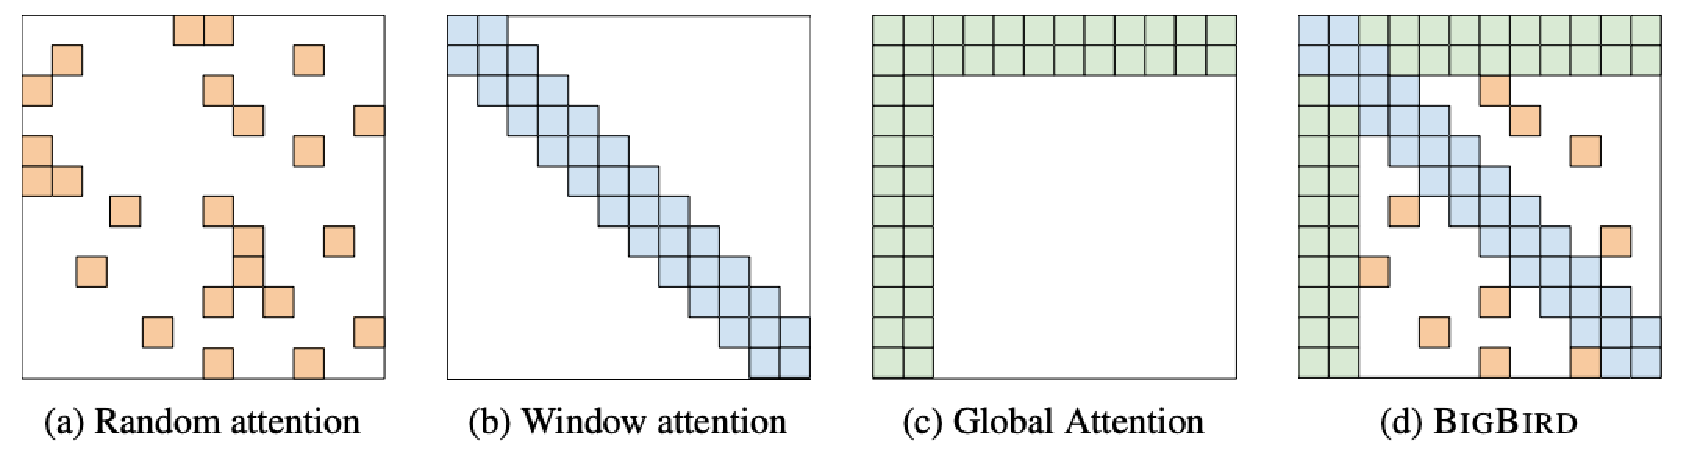
\includegraphics[width=\textwidth]{images/chapter2/big-bird-attention.pdf}
    \caption{Attention mechanisms used in BigBird. Illustration from \citet{zaheer2020big}.}
    \label{fig:related-long-range-modeling-bigbird-attention}
\end{figure}

The earliest modifications to self-attention involve applying pattern-based methods to sparsify the attention matrix. By computing attention solely on a limited number of query-key pairs, this approach restricts the field of view to specific patterns.
The key idea is to relax the constraint that a single layer needs to aggregate information from any two tokens. Although the attention of each layer is not dense, the receptive field can be increased as multiple layers are stacked. 

As an initial attempt, the Sparse Transformer \citep{child2019generating} introduces a two-dimensional factorization of the attention matrix, where the network can attend to all positions through two steps of sparse attention. Half of the attention heads attend only to preceding elements in the sequence, while the other half attend to predesignated indices spread evenly throughout the sequence. 

% With \textit{dilated window attention}, the window has gaps of size dilation $r$, resulting in a receptive field of $l \times r \times k$ where $l$ is the total number of layers.
Longformer \citep{beltagy2020longformer}, a variant of Sparse Transformer, employs self-attention on both \textit{local} and \textit{global} contexts by introducing three attention patterns: \textit{sliding window attention}, \textit{dilated window attention}, and \textit{global attention}. The key concept underlying the first two patterns is similar to convolution: the most important information is supposedly contained in the neighbourhoods of the tokens \citep{liu2022leveraging}. \textit{Sliding window attention} constrains the field of view for each token to a $k$-sized window centered on the token. Although a token can only attend to itself and its neighbours in a single layer, sliding window attention enables a multi-layer Transformer to achieve a receptive field covering the entire sequence. Due to the need for multiple layers to incorporate information from the complete sequence, the sliding window can be \textit{dilated} to increase the receptive field without increasing computation. However, dilated sliding window attention alone does not suffice to produce task-specific representations: some tokens are so important that it is highly beneficial that each token is connected to them and conversely (\textit{e.g.}, through a single layer, the \texttt{[CLS]} token needs to have access to all input tokens for sequence classification tasks). \textit{Global attention} addresses this issue by allowing $s$ fixed, user-defined tokens to attend to every other token and vice-versa, enabling the model to learn task-specific representations. 

BigBird \citep{zaheer2020big} extends Longformer by adding \textit{random pattern attention}, which allows every token to attend to $r$ tokens chosen randomly, where $r$ is a small constant number. The intuition behind this mechanism is that the path lengths in a randomly connected graph are on average logarithmic. The attention mechanisms employed in BigBird are depicted in Figure~\ref{fig:related-long-range-modeling-bigbird-attention}.

The \ac{ETC} model \citep{ainslie2020etc} represents another iteration within the Sparse Transformer family. It introduces a novel \textit{global-local} attention mechanism, encompassing four distinctive components: \textit{global-to-global}, \textit{global-to-local}, \textit{local-to-global}, and \textit{local-to-local} attentions. In addition to the original input, \ac{ETC} integrates $n_g$ auxiliary tokens at the beginning of the sequence, functioning as global tokens for participating in global-to-* and *-to-global attention processes. The local-to-local component uses a sliding window of size $k$. Notably, \ac{ETC}'s approach closely resembles that of Longformer in its incorporation of global auxiliary tokens, which function as trainable parameters and can be interpreted as a form of model memory that pools across the sequence to collect global sequence information. 

The Sparse Transformer has a loglinear time and memory complexity, while Longformer, BigBird, and \ac{ETC} operates with a linear time and memory complexity. None of these models introduces new parameters beyond the Transformer model. Given the global attention mechanism, computing causal masks (Section~\ref{subsubsection:related-pretrained-language-models-unidirectional-sa}) becomes unfeasible. As a result, the attention mechanisms employed by Longformer, BigBird, and \ac{ETC} are unsuitable for use in an autoregressive setting. Nevertheless, they can be effectively applied in sequence-to-sequence modeling, employed in the encoder while standard self-attention is retained in the decoder. Both Longformer and BigBird, as well as \ac{ETC}, have the capacity to handle up to 4,096 tokens.

\subsubsection{Recurrence}
\label{subsubsection:related-long-range-modeling-recurrence}

Recurrence and compressed memory approaches incorporate \textit{segment-level recurrence} into Transformer models to lengthen their attention span. The underlying concept of segment-based recurrence methods is to consider blocks of local receptive fields by chunking the input sequence into segments, and then process them in series via recurrence, as in \acp{RNN}.

Rather than attempting to reduce the cost of self-attention, \citet{dai2019transformer} take inspiration from \acp{RNN} and propose Transformer-XL, a causal language model that introduces a segment-based recurrence mechanism to connect adjacent segments. In Transformer-XL, segments are sequentially fed to the model, and tokens within a segment attend to the rest of the segment \textit{and} to the hidden states of the previous segment. Hence, after the first segment, tokens in subsequent segments will always have an immediate context size of $n$. By stacking multiple attention layers, the receptive field can be increased to multiple previous segments. In addition, this recurrence mechanism provides context for tokens in the beginning of a new segment. 
 
XLNet \citep{yang2019xlnet} leverages both autoregressive and bidirectional language modeling. Unlike traditional autoregressive models that rely on fixed forward/backward factorization orders, XLNet maximizes the expected log likelihood of a sequence across all possible permutations of factorization orders. This approach allows each position in the sequence to consider tokens from both left and right, creating a bidirectional context. Additionally, XLNet incorporates the segment recurrence mechanism and relative encoding scheme of Transformer-XL during pre-training. This integration empirically improves the model's performance, specifically for tasks involving long text sequences. 

\subsubsection{Approximating the Attention Mechanism}
\label{subsubsection:related-long-range-modeling-approx}

Another approach to improve the efficiency of Transformer models is to approximate the self-attention mechanism through techniques such as \textit{learnable patterns}, \textit{low-rank approximation}, or \textit{kernelization}. The idea revolves around mathematically redefining the self-attention mechanism, which eliminates the need to explicitly compute the $n \times n$ matrix.

% If $\bm{K} = \bm{Q}$ then only the similarity of query vectors to each other has to be computed. 
Reformer \citep{kitaev2020reformer} uses learnable patterns that enable the model to learn the access pattern in a data-driven fashion. Learnable patterns facilitates a more global view of the sequence while maintaining the efficiency benefits of fixed patterns approaches. Reformer introduces \ac{LSH} attention, a novel attention mechanism that consists in sharing parameters between $\bm{Q}$ and $\bm{K}$, and clustering tokens into chunks. This concept is rooted in the idea that if the sequence is long, $\text{softmax}(\bm{Q}\bm{K}^{\top})$ only puts significant weight on very few key vectors for each query vector. Hence, given a query $\bm{q}$, $\text{softmax}(\bm{qK})$ can be approximated by using only the keys that have a high cosine similarity with $\bm{q}$. Using the \ac{LSH} algorithm, query vectors are hashed into buckets of similar vectors. Attention is then computed among each bucket. If the bucket size is appropriately selected, the time and memory complexity of Reformer is $\mathcal{O}(n \log n)$. 
% Reformer can be used in both bidirectional and autoregressive settings. 

% In a high-rank matrix, no particular dimension has much more information than any other. Conversely, most of the information in a low-rank matrix is concentrated in very few dimensions, meaning that most of the dimensions are redundant. The core idea behind Linformer \citep{wang2020linformer} is to approximate the self-attention matrix with a lower rank matrix. 
% The projected matrices $k \times d$ can be viewed as producing a set of $k$ pseudo-tokens that summarize the sequence — each of these pseudo-tokens indicates how highly a given filter activates on average when multiplied with the full sequence of corresponding representations.
Rather than approximating the softmax operator, alternative approaches have aimed to approximate the full attention mechanism using low-rank approximations. In Linformer \citep{wang2020linformer}, the keys and values are projected to a lower-dimensional representation $k \times d$, where $k < n$. As $k$ does not depend on the sequence length $n$, the time and memory complexity of Linformer is linear. There is only a minimal parameter costs of the Linformer due to the extra $nk$ length projections. If $k$ is sufficiently small, there is negligible parameter costs incurred. 

% To evaluate Linformer, \citet{wang2020linformer} used sentiment classification \citep{maas2011learning, socher2013recursive}, \ac{NLI} \citep{wang2018glue} and textual similarity \citep{wang2017bilateral} tasks. 

% Because projecting on the length dimension $n$ causes mixing of sequence information, it is non-trivial to maintain causal masking and/or prevent mixing of past and future information when computing attention scores. Hence, Linformer's attention approximation cannot be used in an autoregressive setting.


To estimate standard full-rank-attention Transformers without relying on any prior such as sparsity or low-rankness, \citet{choromanski2020rethinking} generalize Linformer by proposing a kernel-based approach that uses a generalized attention framework to approximate any attention matrix. 
% The attention matrix $\text{softmax}(\bm{Q}\bm{K}^{\top})$ can be approximated using lower-rank randomized matrices $\bm{Q'}$ and $\bm{K'}$ where the rows encode positive-valued nonlinear functions of the original $\bm{Q}$ and $\bm{K}$. This approximation allows to store the implicit attention matrix $\bm{A}$ with linear memory complexity. Additionally, this framework facilitates the creation of a diverse range of attention mechanisms by leveraging various similarity measures (kernels). 
% To obtain a linear time complexity, matrix multiplications are rearranged: instead of multiplying $\bm{A}$ with $\bm{V}$ to obtain the final $n \times d$ matrix, $\bm{K'}^{\top} \in \mathbb{R}^{k \times n}$ is first multiplied with $\bm{V} \in \mathbb{R}^{n \times d}$, and $\bm{Q'} \in \mathbb{R}^{n \times k}$ is multiplied with the resulting matrix $\bm{K'}^{\top} \bm{V} \in \mathbb{R}^{k \times d}$. This framework allows to create a broad class of attention mechanisms based on different similarity measures (kernels). 

% Performer was evaluated as an encoder-only model on protein modeling \citep{uniprot2019uniprot} and image generation \citep{parmar2018image} tasks. 

Reformer can be used in both bidirectional and autoregressive settings. In Linformer, projection along the length dimension $n$ induces the mixing of sequence information. Similarly, the randomized feature map and the approximations involved in the kernel-based approach might not inherently preserve the sequential order required for causal masking. Therefore, it is non-trivial to maintain causal masking and/or prevent mixing of past and future information when computing attention in both Linformer and Performer. Consequently, both Linformer's and Performer's attention approximations are unsuitable for deployment in an autoregressive setting. Similar to Longformer, BigBird, and \ac{ETC}, these attention mechanisms are restricted to the encoder of the Transformer.

\subsection{Benchmarking Long-range Models}

The broad array of efficient Transformers that has emerged to address the challenge of long-range modeling have been mostly evaluated using differents sets of downstream tasks and datasets. Longformer and BigBird were evaluated on question answering \citep{yang2018hotpotqa, welbl2018constructing} and text classification \citep{maas2011learning, kiesel2019semeval}. \ac{ETC}'s evaluation extends to information extraction tasks \citep{xiong2019open}. XLNet's performance is assessed using machine reading comprehension \citep{lai2017race} and document ranking\footnote{\url{https://lemurproject.org/clueweb09/}}. Linformer is evaluated on easier tasks such as sentiment classification \citep{maas2011learning, socher2013recursive}, \ac{NLI} \citep{wang2018glue} and textual similarity \citep{wang2017bilateral}, where simpler models such as \acp{CNN} perform well. On the other hand, the Sparse Transformer, Reformer, and Performer have their performance assessed on image generation tasks \citep{parmar2018image}. The large diversity of tasks and datasets used complicates the comparison of models and the assessment of their relative strengths and weaknessses. 

Furthermore, intrinsic metrics such as perplexity or \ac{BPC} are widely used to assess the performance of efficient Transformers. However, an increasing amount of literature shows that predicting the next token is mostly a local task that does not require modeling long-range dependencies \citep{khandelwal2018sharp, sun2021long}. 

In this section, we describe unified benchmarks designed to shed light on the ability of these architectures to reason in long-context scenarios, and study their performance in handling \ac{NLP} tasks.

\subsubsection{Long-Range Benchmarks}

\citet{tay2020long} introduce a systematic and unified benchmark, \ac{LRA}, designed to evaluate the ability of a model to reason in long-context scenarios. This benchmark is a suite of tasks with sequences ranging from 1,000 to 16K tokens, encompassing various data types and modalities (text, natural and synthetic images, mathematical expressions). This benchmark was created based on a set of specific requirements and criteria. First, \ac{LRA} is general: all long-range Transformer models are applicable to the tasks. The tasks are intentionally designed to promote simple models rather than cumbersome pipelined approaches. Furthermore, the tasks are crafted to be challenging enough to ensure there is room for improvement. The input sequences are reasonably long, and the set of tasks allows to assess different capabilities of models. Finally, \ac{LRA} is deliberately non-resource intensive and accessible. However, only two out of these five tasks involve natural language, restricting the relevance of \ac{LRA} for \ac{NLP}. Furthermore, \ac{LRA} artificially increases the length of natural language sequences through character tokenization, and truncates each example at 4,000 characters, equivalent to less than 1,000 words. This exempts models from dealing with the complex long-range interactions present in long texts.

% \ac{LRA} contains five classification tasks. In \textit{Long ListOps}, sequences with a hierarchical structure and mathematical operators are given as input and the model has to predict the mathematical result of the sequence as a classification task. The goal is to evaluate the ability to model hierarchically structured data while handling long contexts. 
% In the \textit{Character-level Sentiment Analysis} task, the model is provided with character-level IMDb reviews \citep{maas2011learning} and has to classify them into positive or negative. This task benchmarks the ability of the model to deal with compositionality as it is required to compose characters into words, and words into higher-level phrases.
% Given two documents from the ACL Anthology Network \citep{radev2013acl} represented as character-level sequences, the \textit{Character-level Document Relatedness} task consists in predicting whether these documents are related. This task assesses the capability of a model to compress long sequences into representations suitable for similarity-based matching. As previously, the character level setup challenges the model to compose and aggregate information over long contexts.
% Using the CIFAR-10 dataset \citep{krizhevsky2009learning}, the \textit{Image Classification on sequences of pixels} task requires the model to learn the 2D spatial relations between input pixels, while presented as a 1D sequence of symbols.
% In \textit{Pathfinder}, the model is given a sequence of pixels and has to predict whether two points are connected by a path. A more challenging version with extreme lengths, \textit{Pathfinder-X}, evaluates if the same algorithmic challenges bear a different extent of diffculty when sequence lengths are much longer.

% However, only two out of these five tasks involve natural language, restricting the relevance of \ac{LRA} for \ac{NLP}. Furthermore, \ac{LRA} artificially increases the length of natural language sequences through character tokenization, and truncates each example at 4,000 characters, equivalent to less than 1,000 words. This exempts models from dealing with the complex long-range interactions present in long texts.

To extend evaluation beyond sentences and paragraphs, \citet{shaham2022scrolls} propose \ac{SCROLLS}, an \ac{NLP} benchmark featuring datasets with long texts, ranging from an average of 1,700 words to over 51,000. \ac{SCROLLS} consists of seven datasets covering various domains and tasks: summarization from government reports (\textit{GovReport}), TV shows transcripts (\textit{SummScreenFD}), and meetings (\textit{QMSum}), question answering from scientific articles (\textit{Qasper}), books (\textit{NarrativeQA}), and stories (\textit{QuALITY}), and \ac{NLI} from non-disclosure agreements (\textit{Contract NLI}). Every task is reformulated as a sequence-to-sequence problem for a simple unified format. \ac{SCROLLS} presents a challenge not only due to the length of its inputs but also because it requires models to process long-range interactions across different sections. 

\subsubsection{On the Effectiveness of Long-range Models for NLP Tasks}

To validate the effectiveness and long-range ability of long-range Transformers on language tasks and uncover the underlying factors behind model behaviors, \citet{qin2022nlp} benchmark different long-range Transformer models for \ac{NLP} tasks characterized by long sequences. Five complex, long-text \ac{NLP} tasks are considered, covering a wide spectrum of typical language scenarios: token/span-level prediction, sequence-level classification, and sequence-to-sequence generation.

% When there is no guiding text (\textit{e.g.}, in the case of coreference resolution), setting all tokens as global reintroduces quadratic complexity.
Longformer and BigBird are used to assess the performance of sparse pattern approaches (Section~\ref{subsubsection:related-long-range-modeling-sparse}). In coreference resolution, which consists in identifying mention spans and clustering them into entities, \citet{qin2022nlp} find that using larger sliding windows can be advantageous, but this advantage tends to level off or even decline after a certain point. In tasks where the quantity of guiding text, \textit{i.e.}, specific textual information provided explicitly to guide the model's behavior, is limited—such as questions in question answering—using them as global tokens can enhance attention and substantially improve overall performance. Additionally, \citet{qin2022nlp} find a connection between long-range attention, global tokens, and the selectivity of sequence-to-sequence problems, which ultimately enhances the decoding process. Globally, the authors show that pattern-based methods, despite being a widely adopted approach, do not effectively capture long distance information.

The effectiveness of recurrence-based methods (Section~\ref{subsubsection:related-long-range-modeling-recurrence}) is evaluated using XLNet. In various tasks, \citet{qin2022nlp} show that the memory of recurrence models tends to enhance performance, demonstrating the advantage of using past hidden states in Transformers. Nevertheless, XLNet falls short in maximizing the potential of past tokens, as it gives relatively less attention to distant information. This could be attributed to XLNet's pretraining objective of predicting masked tokens, which does not consistently require long-range context \citep{sun2021long}. Moreover, the application of the stop-gradient technique might impede the model's ability to efficiently focus on memories.

Performer is used as a kernel-based model (Section~\ref{subsubsection:related-long-range-modeling-approx}). It is found that the approximation technique of Performer demonstrates strong performance with shallow networks. However, when applied to deeply stacked Transformer layers, it encounters significant  error accumulation issues. This leads to a notable drop in performance, which is considered unacceptable even for the base version of Transformer encoders. 

Drawing from their discoveries, \citet{qin2022nlp} offer a few recommendations. For typical tasks like sequence classification or token-level prediction, it remains effective to divide inputs into chunks and use short-range Transformer models. In cases where explicit guiding text such as queries is available, models based on sparse patterns and featuring a global token mechanism are preferable. For sequence-to-sequence problems, leveraging long-range Transformers with pre-trained checkpoints yields superior performance. 

\subsection{Conclusion}

The exploration of long-range modeling has been marked by continuous efforts to reduce the cost of Transformers to efficiently model long texts. The quest for ideal long-range models demands finding an equilibrium. These models should address the quadratic issue of Transformers, showcase universality by performing well across most tasks, and remain simple without unnecessary hard-coding or engineering complexities. There should be no compromise between speed and memory efficiency, and they should be able to seamlessly integrate with TPUs and accomodate causal masking. 

The research conducted in this PhD thesis is in line with the continuous efforts to model long texts efficiently. Chapter~\ref{chapter:skim-attention} contributes to research on efficient long-range modeling by proposing a sparse attention pattern based on the layout of documents, introducing a novel approach to alleviate the computational burden associated with long-range modeling. Acknowledging the importance of document structures in guiding summary generation, Chapter~\ref{chapter:loralay} integrates layout information into existing long-range models \citep{zaheer2020big}, thereby improving summarization of long documents and highlighting the significance of layout information in capturing long-range dependencies. 

\section{Conclusion}

Transformer-based Pretrained Language Models have brought significant breakthroughs to \ac{NLP} \citep{devlin2018bert, lewis2019bart, brown2020language}. Despite remarkable achievements, the quadratic complexity of the Transformer hinders their effective application to long texts. In tasks involving long texts, many works tend to apply the same approaches used for processing shorter ones (\textit{e.g.} truncating or chunking) without addressing the challenges specific to long texts (\textit{e.g.}, long-range dependencies and complex hierarchical structures). While various Transformer variants have been proposed to efficiently model long texts, there is currently no variant that can be confidently identified as having effectively addressed the efficiency challenges in Transformers while preserving performance comparable to that obtained with full self-attention.

The next chapter will address the applicative scope of this PhD thesis: Document Understanding. Notably, the prevailing approach in solving document understanding tasks involves leveraging Pre-trained Language Models to jointly learn text and multimodal information. 

% Our contributions in this PhD thesis leverage the modeling capabilities of Transformer-based Pre-trained Language Models to effectively represent documents. In addition, we employ existing long-range models as a foundation to efficiently address the challenges posed by long documents. 

\acresetall

